% PREAMBLE
\documentclass[12pt, twoside]{report}
\raggedbottom

% Add your useful packages here
\usepackage[utf8]{inputenc}
\usepackage{amsmath}
\usepackage{amsfonts}
\usepackage{amssymb}
\usepackage{csquotes}
\usepackage{graphicx}
\usepackage[main=english,vietnamese]{babel}
\usepackage[a4paper, top=1in, bottom=0.8in, left=1in, right=1in]{geometry}
\usepackage{fancyhdr}
\usepackage{float}
\usepackage{array}
\usepackage{booktabs}
\usepackage{url}
\usepackage{textgreek}
\usepackage{algorithm}
\usepackage{algpseudocode}
\usepackage{indentfirst}     % Thụt cả đoạn đầu sau section
\setlength{\parindent}{0.5 cm}
\setlength{\parskip}{0pt}
\usepackage{multirow}
\usepackage{tikz}
\usetikzlibrary{arrows.meta, positioning, shapes.geometric, fit}



% Include graphics path, you have to put your images into images/ folder, and only refer their name when adding them
\graphicspath{{images/}}


% BODY
\begin{document}
	\pagenumbering{arabic}
	\begin{titlepage}
		\centering
		\vspace{1 cm}
		\textbf{VIETNAM NATIONAL UNIVERSITY -- HO CHI MINH CITY}\par \textbf{
		INTERNATIONAL UNIVERSITY}\par \textbf{SCHOOL OF COMPUTER SCIENCE AND ENGINEERING}\par

		\vspace{2 cm}
        
\includegraphics[width=0.4\textwidth]{IU.png}


		\vspace{2 cm}
		\textbf{\Large A DEEP LEARNING APPROACH FOR} \par \textbf{\Large ARTWORK RECONSTRUCTION}

		\vspace{2cm}
		By \par \textbf{Ngo Thi Thuong}

		\vspace{2cm}
		\textit{A thesis submitted to the School of Computer Science and Engineering \\ in partial
		fulfillment of the requirements for the degree of \\ Bachelor of Computer Science}

		\vspace{2cm}
		\text{Ho Chi Minh City, Vietnam} \par 2026

		\newpage
		% Signature Page (ii, not printed)
		\centering
		\vspace*{1cm}

		\textbf{\large A DEEP LEARNING APPROACH FOR ARTWORK RECONSTRUCTION}\par
		\vspace{3cm}

		\noindent
		\begin{minipage}[t]{0.45\textwidth}
			\centering
			\textbf{APPROVED BY: Supervisor}\par
			\vspace{2.2cm}
			\underline{\hspace{6cm}}\par
			\vspace{0.3cm}
			Le Thi Ngoc Hanh, Ph.D
		\end{minipage}
		\hfill
		\begin{minipage}[t]{0.45\textwidth}
			\centering
			\textbf{APPROVED BY: Committee}\par
			\vspace{2.2cm}
			\underline{\hspace{6cm}}\par
			\vspace{0.3cm}
			Le Thi Ngoc Hanh, Ph.D
		\end{minipage}

		\thispagestyle{empty}
	\end{titlepage}

% =========================
% Optional: Acknowledgments
% =========================
\chapter*{Acknowledgments}
\addcontentsline{toc}{chapter}{Acknowledgments}
I would like to express my sincere gratitude to my advisor, Le Thi Ngoc Hanh, Ph.D, for her invaluable guidance, patience, and continuous support throughout the development of this thesis. Her insightful comments and constructive feedback helped me clarify difficult ideas, refine my research direction, and improve both the technical and academic quality of this work. During the most challenging stages of the research, when repeated experimentation and revision were necessary, her encouragement and advice gave me the motivation to persist, learn independently, and gradually strengthen the proposed approach. I deeply appreciate her willingness to discuss my questions and provide direction whenever I encountered difficulties.

I would also like to thank the Department for providing the necessary resources and a supportive academic environment that enabled me to carry out this research effectively. In particular, I am grateful for the access to computing facilities and research infrastructure, which played an important role in the implementation and evaluation of the image inpainting models presented in this thesis.

This research was also supported by the Central Interdisciplinary Laboratory in Electronics and Information Technology (AI and Cooperation Robot), International University -- VNU-HCM. I would like to sincerely thank the laboratory for providing the computing machines and experimental support that were essential for training, testing, and completing this thesis.

I am especially grateful to my family for their unconditional love, understanding, and encouragement throughout my study. I would like to thank my mother, my sisters, and all members of my family for supporting me both emotionally and practically during the demanding period of completing this thesis. Their trust, patience, and constant encouragement gave me the strength to continue working through difficulties and remain committed to finishing this research.

I am also thankful to my friends and to everyone who offered encouragement, advice, and companionship during my studies. Their support, whether through discussion, motivation, or simple words of encouragement, contributed meaningfully to my ability to complete this work.

I am truly grateful to everyone who, directly or indirectly, contributed to the completion of this thesis.

\thispagestyle{empty}
% Table of Contents, List of Figures, List of Tables
\tableofcontents

\listoffigures
\addcontentsline{toc}{chapter}{List of Figures}

\listoftables
\addcontentsline{toc}{chapter}{List of Tables}



% =========================
% Abstract
% =========================
\chapter*{Abstract}
\addcontentsline{toc}{chapter}{Abstract}
Artworks and cultural heritage images often suffer from cracks, stains, missing regions, and other aging-related damage. Digital restoration offers a non-invasive way to explore possible reconstructions without altering the original object. Among digital restoration techniques, image inpainting is especially relevant because it reconstructs missing content from surrounding visual context. Most modern inpainting methods, however, are developed mainly for natural images. As a result, they do not fully address the stricter requirements of artwork reconstruction, where structure, color harmony, brushstroke continuity, and style consistency must all be preserved.

This thesis studies artwork reconstruction through a deep learning framework for portrait artworks with damaged facial regions. The thesis title is intentionally broad, but the practical focus is narrower. It centers on painted portraits because errors in the eyes, nose, mouth, and facial contour are immediately noticeable and can quickly reduce the credibility of a restored result. Existing restoration pipelines may produce acceptable completions in less sensitive regions. Face-dominant damage is more difficult because it requires painterly consistency and accurate facial arrangement at the same time.

To address this problem, the thesis develops the Portrait Artwork Reconstruction Framework (PARF). PARF follows a coarse-to-refinement design. The first stage estimates the global facial layout. The second stage refines local detail, boundary continuity, and painterly appearance. The framework also integrates residual adapter enhancement in the deeper transformer stages, deterministic latent guidance, and a frequency-aware training design based on Focal Frequency Loss (FFL). A curated portrait-artwork dataset and fixed evaluation masks are prepared to support consistent qualitative and quantitative assessment.

The experimental evaluation uses PSNR, SSIM, and LPIPS, together with visual comparison against selected transformer and diffusion baselines. The results show that PARF improves reconstruction fidelity and perceptual quality under the selected evaluation protocol. It achieves the highest PSNR and the lowest LPIPS among the compared methods. The qualitative results further show better facial coherence, smoother integration around damaged regions, and stronger preservation of painterly appearance in representative portrait cases. The study also identifies a clear limitation under severe face-dominant occlusion, where too much structural evidence is removed. Overall, the thesis shows that a modern deep learning framework can be adapted in a meaningful way for non-invasive portrait artwork reconstruction, while also clarifying the cases in which the current design becomes less reliable.

\iffalse

This thesis investigates image inpainting specifically in the context of artwork restoration. The study focuses on evaluating and adapting modern deep learning-based inpainting approaches to address the unique challenges posed by artistic images, including irregular damage patterns, complex brushstroke textures, and high-resolution requirements. In particular, this work explores transformer-based inpainting models, with emphasis on the Mask-Aware Transformer (MAT), due to their ability to capture long-range dependencies and maintain global structural coherence under large missing regions.
A curated dataset of artworks is constructed using publicly available painting collections, and restoration-inspired mask generation strategies are designed to simulate realistic artwork degradation. The proposed experimental pipeline includes dataset preprocessing, mask generation, model fine-tuning, and systematic evaluation. Model performance is assessed using quantitative metrics such as PSNR, SSIM, LPIPS, and FID, together with qualitative visual evaluation criteria relevant to artwork restoration, including structural fidelity, brushstroke continuity, color harmony, and overall perceptual quality.

Experimental results indicate that transformer-based inpainting models provide improved visual coherence and texture reconstruction compared to traditional and baseline learning-based methods, particularly for large and irregular missing regions. Qualitative comparisons further demonstrate smoother tonal transitions, better preservation of artistic style, and more plausible restorations suitable for supporting conservation analysis. The findings of this study highlight the potential of advanced image inpainting techniques as effective tools for digital artwork restoration and provide insights into adapting general-purpose inpainting models for culturally and artistically sensitive applications.

\fi

\textbf{Keywords:} image inpainting, artwork reconstruction, portrait artwork restoration, PARF, deep learning framework, Focal Frequency Loss, perceptual evaluation



\chapter{Introduction}

\section{Background}
The preservation and restoration of artworks play an important role in maintaining cultural and historical heritage. Oil paintings, classical portraits, and artistic illustrations often deteriorate over time. The causes are varied. They include aging, environmental conditions, physical damage, and improper storage. Common defects include cracks, missing paint regions, stains, scratches, and partial loss of visually important elements such as faces.

With the development of digital imaging technologies, artworks are increasingly digitized at high resolution for archival, research, and exhibition purposes. Digital restoration has therefore become an important complement to manual restoration. It allows damaged artworks to be reconstructed virtually, without physical intervention. This gives conservators and researchers a safer environment in which to test restoration hypotheses and inspect possible outcomes.


\begin{figure}[htbp]
  \centering
  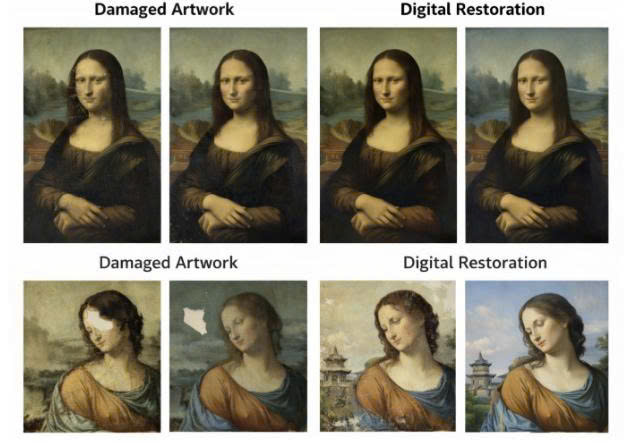
\includegraphics[width=0.80\linewidth]{fig1_1_damaged_vs_restored.jpg}
  \caption{Examples of damaged artworks and corresponding digital restoration results produced by an image inpainting framework.}
  \label{fig:damaged_restored}
\end{figure}

Figure~\ref{fig:damaged_restored} illustrates the general motivation of the thesis by showing the transition from damaged artwork content to a digitally restored result. The damaged inputs contain visually disruptive missing or corrupted regions that interrupt the continuity of the original painting. The restored examples show the expected role of an inpainting framework: the missing region should be filled in a way that is visually compatible with the surrounding colors, texture, and structure. In the context of this thesis, the figure emphasizes that digital artwork reconstruction is not simply pixel replacement, but a restoration-oriented process that must preserve the visual identity and artistic appearance of the original work.

In practice, artwork damage patterns are diverse. Figure~\ref{fig:damage_taxonomy} summarizes typical damage types, including crack networks, paint loss, stains, and occlusions. In real restoration, these patterns are often irregular and large, making the reconstruction task challenging.

\begin{figure}[H]
  \centering
  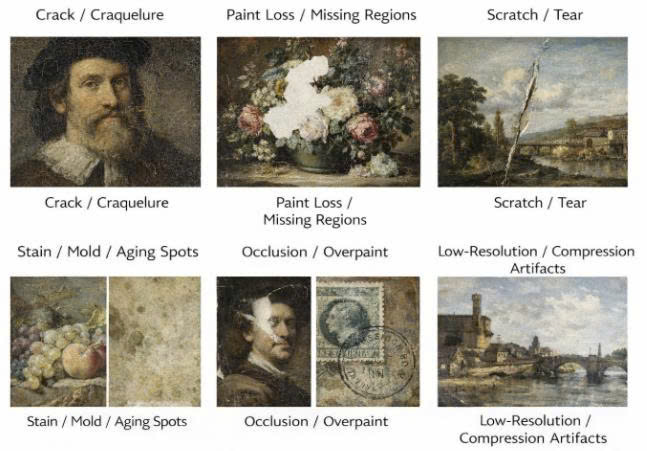
\includegraphics[width=0.88\linewidth]{fig1_2_damage_taxonomy.jpg}
  \caption{Taxonomy of common damage types in artworks and artistic images.}
  \label{fig:damage_taxonomy}
\end{figure}

Figure~\ref{fig:damage_taxonomy} categorizes the main forms of degradation considered in artwork restoration. Thin cracks and scratch-like defects mainly require local continuity, while larger paint-loss regions require the model to infer missing semantic content from surrounding evidence. Stains and occlusions introduce an additional difficulty because the corrupted region may still contain misleading visual information rather than a clean missing hole. This taxonomy is useful for the thesis because it clarifies why a restoration framework must be robust to both fine-scale damage and large irregular masks, especially when damage overlaps sensitive portrait regions.

Image inpainting is a core technique in digital restoration. Its goal is to fill missing or corrupted regions so that the completed image remains visually plausible and consistent with the surrounding context. Artwork restoration is stricter than natural-image restoration. It must preserve stylistic coherence, brushstroke continuity, and compositional balance. In portrait artworks, face regions are especially sensitive. Small errors in the eyes, mouth, or facial contour can quickly reduce realism and harm the perceived authenticity of the result.

This distinction is important for the positioning of the thesis. Although the title remains broad, the practical focus is narrower: portrait artworks in which damage overlaps semantically important facial components. In many categories of artwork, approximate completion may still look acceptable at a general level. Portrait restoration is less forgiving. Even small inconsistencies in the eyes, nose, mouth, or overall facial proportion are easy to notice. For that reason, portrait artwork reconstruction provides a demanding setting for evaluating whether a modern inpainting framework can move beyond generic visual completion and support a more credible restoration in artistically sensitive regions. The proposed system is referred to throughout this thesis as the Portrait Artwork Reconstruction Framework (PARF).

\begin{figure}[H]
  \centering
  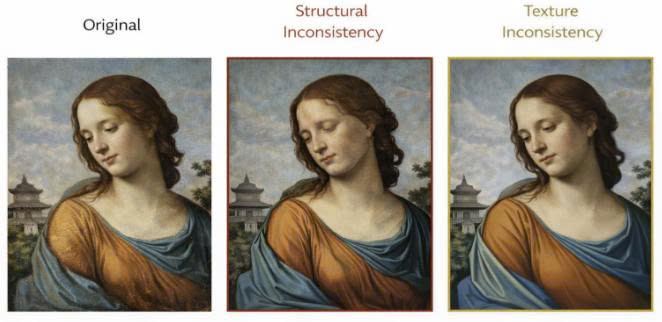
\includegraphics[width=0.88\linewidth]{fig1_3_structure_texture_tradeoff.jpg}
  \caption{Illustration of the structure--texture trade-off in artwork inpainting.}
  \label{fig:structure_texture}
\end{figure}

Figure~\ref{fig:structure_texture} visualizes the central trade-off in artwork inpainting between structural correctness and texture consistency. A restoration may preserve local texture but still fail if facial geometry, contour alignment, or object structure is incorrect. Conversely, a structurally plausible restoration may still appear artificial if the generated region does not match the surrounding brushstroke pattern, color tone, or painterly texture. This trade-off directly motivates the design of PARF, which combines transformer-based structural reasoning with refinement and frequency-aware training to improve both facial coherence and painterly appearance.

From an application perspective, several tool families are already used for digital artwork restoration. Manual editing software provides retouching and content-aware filling functions that are widely adopted in practice. These tools can work well for small defects, but they require substantial manual effort and often struggle with large missing regions or complex artistic textures. More recently, general-purpose AI image generation tools have become capable of regenerating missing image parts and producing visually appealing outputs. Their main objective, however, is broad image synthesis rather than faithful artwork reconstruction. In practice, they may change artistic style, distort facial identity, or introduce semantically inconsistent details. Figure~\ref{fig:tool_comparison} illustrates this contrast between manual editing tools, general AI generation tools, and specialized inpainting frameworks.

\begin{figure}[H]
  \centering
  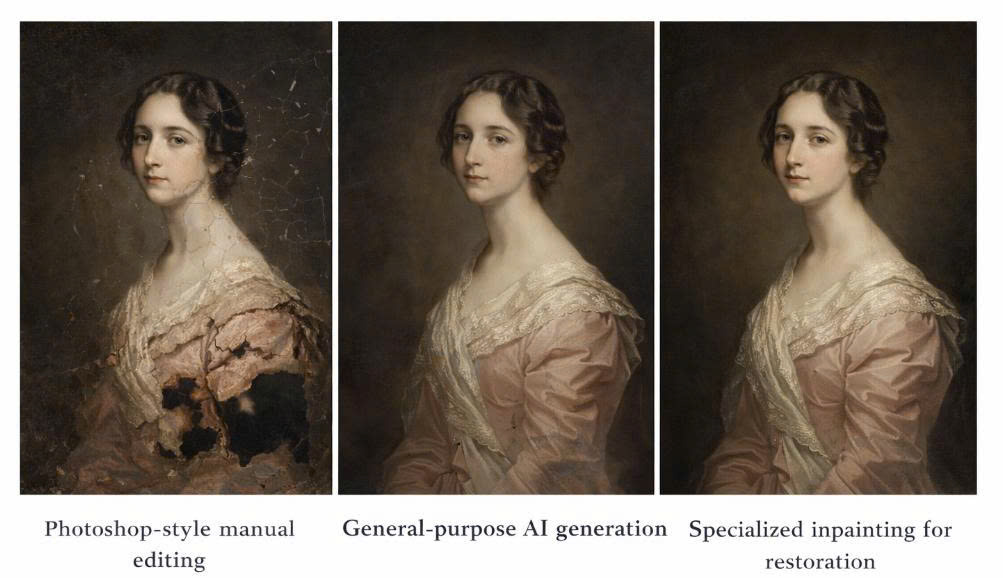
\includegraphics[width=0.92\linewidth]{fig1_4_tool_comparison.jpg}
  \caption{Illustrative comparison of artwork restoration approaches}
  \label{fig:tool_comparison}
\end{figure}

Figure~\ref{fig:tool_comparison} compares three practical directions for digital restoration. Manual editing tools provide strong human control but depend heavily on expert effort and may become impractical when the missing region is large or structurally complex. General AI generation tools can synthesize visually appealing content, but their outputs may not remain faithful to the original artwork because they are optimized for broad image generation rather than restoration constraints. Specialized inpainting frameworks occupy the middle ground: they are designed to use the visible context and mask information directly, making them more suitable for controlled restoration experiments such as the portrait-artwork reconstruction task studied in this thesis.

These limitations motivate research on specialized inpainting frameworks that can handle large and irregular damage while preserving both structure and artistic style. Face-oriented artwork reconstruction is especially important because portrait artworks are common and facial artifacts are highly noticeable. PARF is introduced in this thesis to address this focused restoration setting rather than to serve as a general-purpose image editing tool.

\section{Problem Statement}
Cultural heritage artworks and artistic images are frequently affected by various forms of degradation, including cracks, missing regions, stains, abrasions, and aging artifacts. While traditional manual restoration remains essential for preserving original materials, it is often time-consuming, costly, and carries the risk of irreversible physical intervention. As a result, digital restoration has become an increasingly important complementary approach for conservation planning, documentation, and public dissemination.

Image inpainting has shown promising results in many image restoration tasks. Its goal is to reconstruct missing or corrupted regions by using surrounding visual context. However, most existing methods are developed and benchmarked on natural image datasets, such as photographs of everyday scenes. These methods often assume more regular object structure, more homogeneous textures, and moderate image resolution. Those assumptions do not reflect the characteristics of artistic images very well.

When applied to artwork restoration, conventional inpainting techniques face several critical challenges. First, artistic images exhibit highly distinctive textures, such as brush strokes, canvas grain, and handcrafted patterns, which are difficult to model using generic natural image priors. Second, damage patterns in artworks are often irregular and diverse, ranging from thin craquelure lines to large missing regions, requiring models to handle both fine-scale and large-scale reconstruction simultaneously. Third, digitized artworks are commonly stored at very high resolutions, placing significant computational and memory demands on existing inpainting models.

Recent deep learning inpainting approaches, particularly transformer models, have demonstrated improved capability in capturing long-range dependencies and maintaining global structural consistency. Nevertheless, their effectiveness for artwork restoration has not been thoroughly investigated, especially under realistic restoration conditions involving damage patterns and stylistic constraints specific to artworks.

Even when existing studies or general restoration pipelines produce acceptable results on broader artwork content, portrait artworks remain a particularly difficult subproblem. The reason is not only that faces attract attention. Facial components also encode fine structural relationships that are easily disrupted by inpainting error. A result may look globally plausible at the level of clothing, background, or coarse silhouette and still fail at the portrait level. If the reconstructed eyes, nose bridge, mouth geometry, or facial contour are inaccurate, the restoration becomes unconvincing. This issue is especially important in painted portraits, where the output must preserve painterly style and believable facial anatomy at the same time.

Therefore, the central problem addressed in this thesis is the lack of systematic investigation and adaptation of modern image inpainting methods for artwork restoration, especially for portrait artworks with face-dominant damage. More specifically, there is a need to evaluate whether advanced inpainting models can reconstruct damaged artistic images while preserving structural integrity, texture continuity, and stylistic consistency. It is also necessary to identify the limitations that appear when general-purpose inpainting techniques are applied to culturally and artistically sensitive material. In this study, the most critical question is whether such models can restore damaged facial regions in painted portraits without distorting the eyes, nose, mouth, or overall facial arrangement.

\section{Scope and Research Goal}

\subsection{Project Scope}
This thesis focuses on digital artwork reconstruction, with a particular emphasis on portrait artworks containing human faces. The study investigates image-based restoration only and does not involve any physical, chemical, or material-level restoration of original artworks.

The scope of this thesis includes:
\begin{itemize}
    \item Two-dimensional artistic images, primarily oil paintings and portrait artworks.
    \item Large and irregular missing regions that commonly occur in artwork degradation.
    \item Digital restoration conducted under controlled experimental settings using simulated damage masks.
    \item Evaluation of restoration quality from both perceptual and structural perspectives.
\end{itemize}

This thesis does not aim to design an entirely new inpainting architecture from scratch. Instead, it develops the Portrait Artwork Reconstruction Framework (PARF) by building on a strong transformer-based inpainting foundation and introducing task-oriented adaptations to study its suitability, behavior, and limitations in the context of portrait artwork restoration.

\subsection{Research Goal}
The main goal of this thesis is to investigate the effectiveness of modern image inpainting techniques for restoring human faces in artistic images. Specifically, this study aims to:
\begin{itemize}
    \item Develop and evaluate PARF for artwork restoration scenarios, with a particular focus on portrait artworks.
    \item Evaluate the ability of PARF to preserve facial structure, texture continuity, and artistic style under large missing regions, with particular attention to visually sensitive facial components such as the eyes, nose, mouth, and facial contour.
    \item Analyze the strengths and limitations of PARF in comparison with the original MAT baseline and selected recent inpainting methods.
    \item Provide practical insights into the potential use of AI-based inpainting models as decision-support tools for digital artwork restoration.
\end{itemize}


\section{Structure of the Thesis}

This thesis is organized into five main chapters, each addressing a specific aspect of the research on image inpainting for digital artwork restoration.

\par \hspace{0.5cm} \textbf{Chapter 1 -- Introduction} provides the overall context and motivation of the study. This chapter discusses the importance of artwork restoration in the digital era, common types of damage observed in artistic images, and the limitations of traditional manual restoration methods. Image inpainting is introduced as a key technique for digital restoration, and the technical challenges specific to artistic images are outlined. The chapter then formulates the research problem, defines the objectives and scope of the study, and presents the overall structure of the thesis.

\par \hspace{0.5cm} \textbf{Chapter 2 -- Literature Review} surveys existing research related to image inpainting. The chapter begins with traditional inpainting methods and progresses to deep learning-based approaches. Recent transformer-based and diffusion-based techniques are reviewed in detail, highlighting their strengths and limitations. In addition, real-world applications of image inpainting in artwork restoration are discussed. The chapter concludes with a summary of the chronological evolution of inpainting techniques, supported by a timeline figure illustrating the development of the field.

\par \hspace{0.5cm} \textbf{Chapter 3 -- Methodology} describes PARF, the methodological framework for portrait artwork image reconstruction. This chapter presents the overall restoration pipeline, the main architectural components of the selected inpainting model, and the training objective that guides optimization. The emphasis is placed on how PARF adapts a transformer-based inpainting foundation to better support face-oriented artwork restoration.

\par \hspace{0.5cm} \textbf{Chapter 4 -- Experiments and Results} presents the practical implementation of PARF together with its experimental assessment. The chapter first introduces the implementation details and dataset preparation process, then reports representative restoration results and direct comparison against baseline methods. It further presents metric-based evaluation, checkpoint-based ablation analysis, and a discussion of the observed strengths and remaining limitations of the proposed approach.

\par \hspace{0.5cm} \textbf{Chapter 5 -- Conclusion and Future Work} summarizes the main findings and contributions of the thesis. This chapter also outlines practical directions for future improvement and broader extension. The closing discussion emphasizes the significance of image inpainting techniques in supporting digital artwork restoration.


% ============================================================
% Chapter 2: Literature Review (skeleton; you can expand later)
% ============================================================
% ============================================================
% Chapter 2: Literature Review
% ============================================================
\chapter{Literature Review}

\section{Overview of Image Inpainting Techniques}

Image inpainting refers to the reconstruction of missing or corrupted image regions so that the completed result remains visually plausible and contextually consistent. The task is not limited to filling an empty area. A good restoration must also preserve structure, texture, and local meaning. In artwork restoration, these requirements become stricter. The restored region must remain compatible with artistic style, brushstroke behavior, and compositional intent, while avoiding artifacts that weaken the credibility of the work.

Early inpainting methods relied mainly on hand-crafted priors. Diffusion-based approaches propagate pixel information from known regions into missing areas by enforcing local smoothness constraints. They work reasonably well for small gaps or thin cracks, but they are much less effective for large or highly textured regions~\cite{bertalmio2000inpainting}. Exemplar-based methods later addressed part of this limitation by copying similar patches from intact regions~\cite{criminisi2004exemplar}. Their success, however, depends on the availability of suitable source textures and often breaks down when global semantic consistency is needed. Efficient patch search methods such as PatchMatch made this family of approaches more practical in interactive workflows~\cite{barnes2009patchmatch}.

The introduction of deep learning changed image inpainting from a hand-crafted procedure into a learned generative problem. Convolutional neural networks and GAN-based models improved perceptual quality and made it easier to handle larger missing regions~\cite{pathak2016context,iizuka2017global}. Even so, the local nature of convolution remains a limitation. These models often struggle with long-range dependencies and may produce structural inconsistencies in more complex scenes.

More recent approaches treat image inpainting as a global reasoning problem. Transformer-based models use self-attention to capture long-range contextual relationships and improve structural coherence under large, irregular masks~\cite{zeng2022zits,li2022mat}. In parallel, diffusion-based methods formulate inpainting as a probabilistic denoising process, which supports high-fidelity texture synthesis and multiple plausible restorations~\cite{lugmayr2022repaint,rombach2022ldm}. These developments are especially relevant to artwork restoration, where large missing regions and stylistic consistency are both common challenges.

Based on this perspective, this thesis focuses on modern inpainting paradigms that emphasize global context modeling and robustness to irregular damage.

\section{Traditional Inpainting Methods}

Traditional image inpainting methods represent the earliest attempts to reconstruct missing or damaged image regions. These methods fill corrupted areas through hand-crafted rules and low-level image priors rather than learned visual knowledge. In practice, they rely on local image statistics, continuity assumptions, and patch similarity to propagate plausible content into missing areas.

Early research focused mainly on diffusion-based methods formulated through partial differential equations (PDEs). Bertalmio et al.~\cite{bertalmio2000inpainting} pioneered this direction by drawing an analogy between image inpainting and fluid dynamics. Their method propagates pixel information from the boundary of the missing region into its interior along isophote directions. This strategy is effective for thin cracks and small gaps, but it depends on strong smoothness assumptions. As a result, diffusion-based methods often produce blurred outputs when the missing region becomes large.

To address these limitations, exemplar-based inpainting methods were introduced. Criminisi et al.~\cite{criminisi2004exemplar} proposed a patch-based algorithm that fills missing regions by copying similar patches from known areas. The method balances confidence and data terms so that both structure and texture can be propagated during reconstruction. Although effective when suitable source textures are available, exemplar-based methods may still introduce repetitive artifacts or semantic inconsistencies when unique structures are missing.

Barnes et al.~\cite{barnes2009patchmatch} further improved patch-based inpainting through PatchMatch, a fast approximate nearest-neighbor search algorithm that made interactive applications more practical. Hybrid approaches that combine diffusion and exemplar-based ideas were also explored in later work.

Despite their historical importance, traditional inpainting methods lack high-level semantic understanding and global context modeling. For this reason, they are generally insufficient for complex artwork restoration tasks, especially when the missing region affects semantically important portrait components.

\begin{figure}[H]
    \centering
    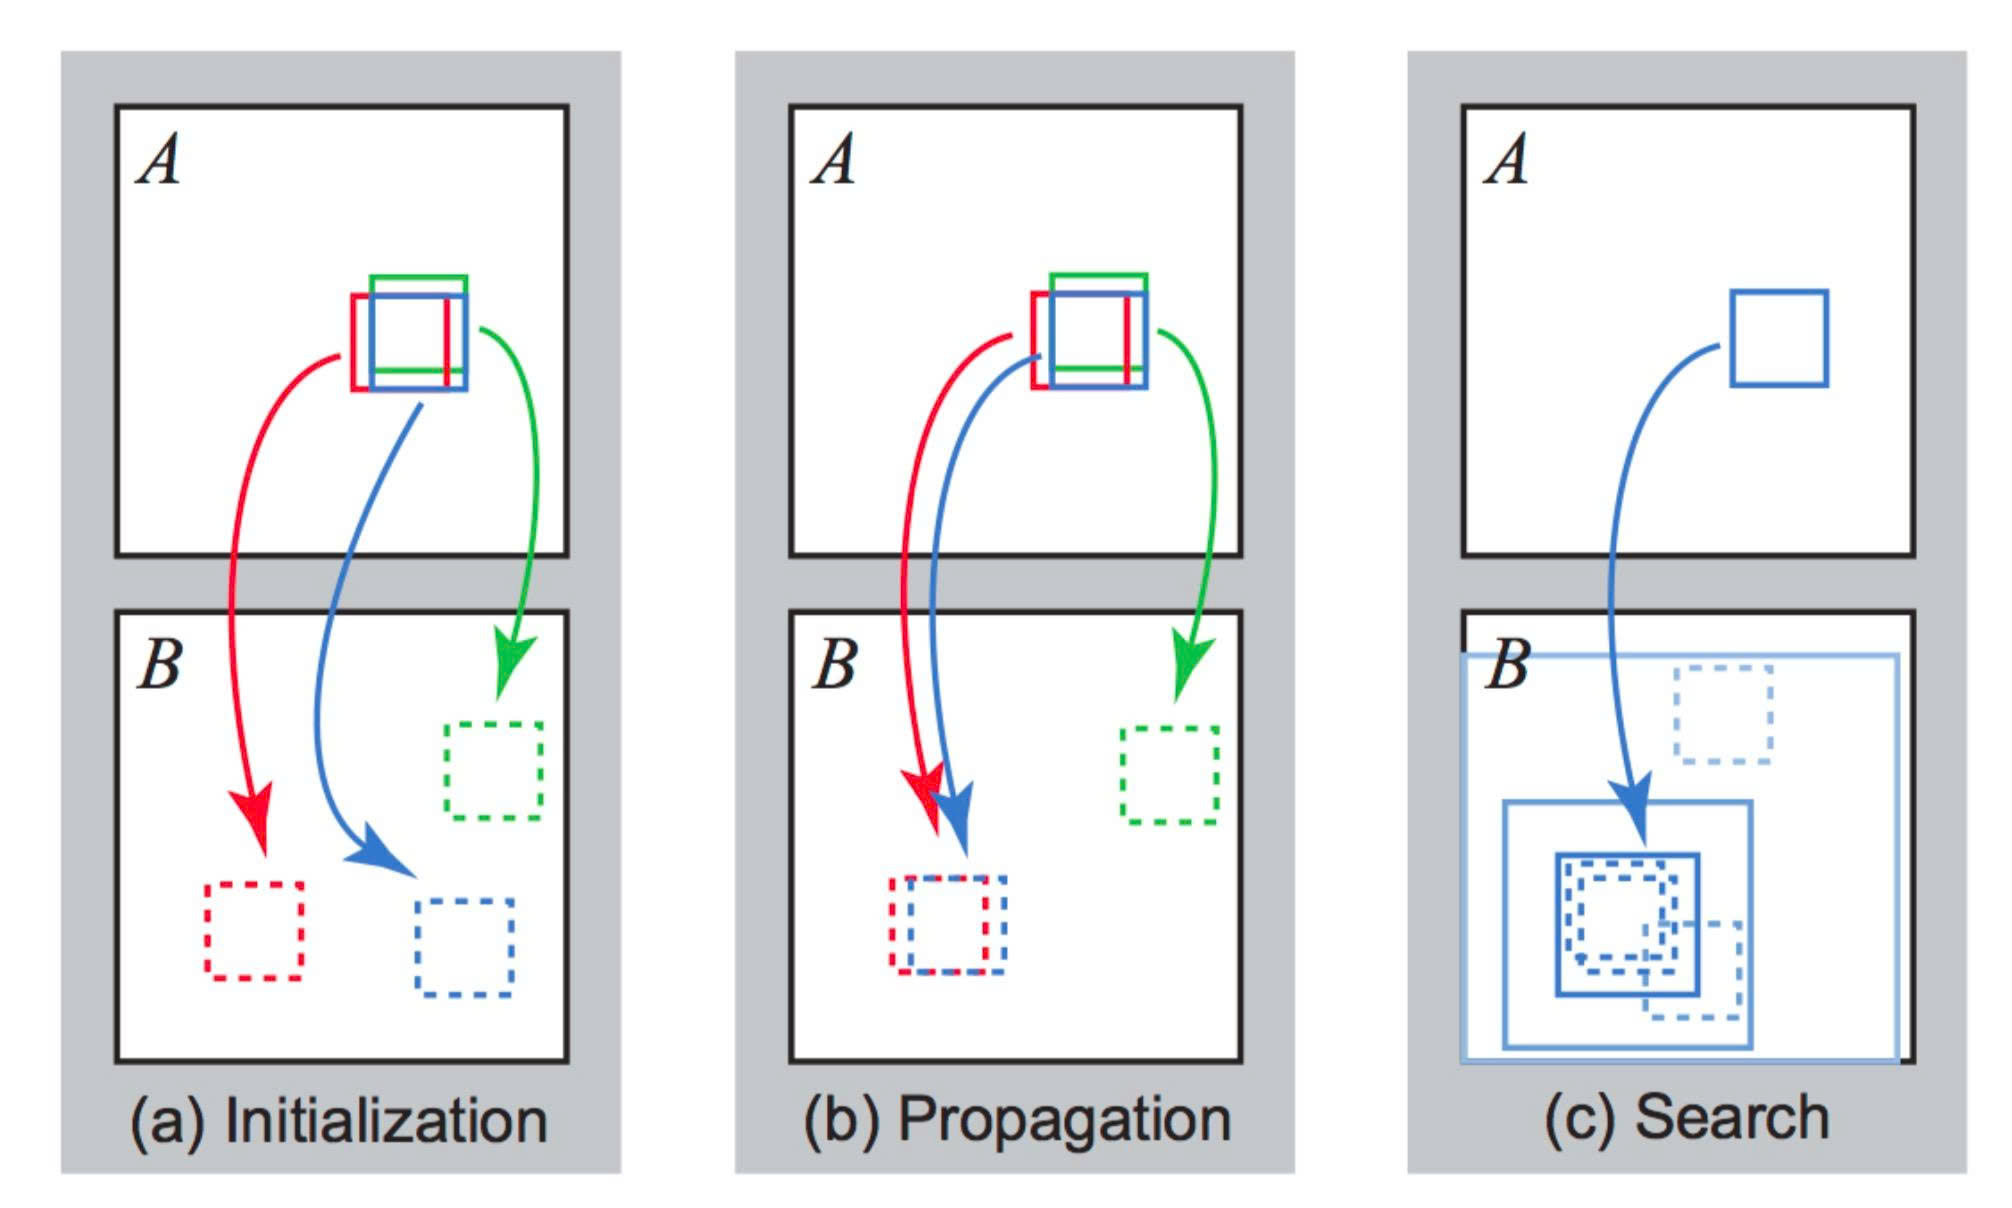
\includegraphics[width=0.75\linewidth]{traditional_inpainting.jpg}
    \caption{Illustration of exemplar-based image inpainting. \textit{Adapted from}~\cite{criminisi2004exemplar}.}
    \label{fig:traditional_inpainting}
\end{figure}

Figure~\ref{fig:traditional_inpainting} illustrates the principle of exemplar-based inpainting. The missing region is completed by searching for similar patches in the known part of the image and copying them into the hole. This strategy works well when the surrounding area contains repeated or similar textures, such as background patterns or relatively homogeneous surfaces. However, in portrait artwork restoration, suitable source patches may not exist for unique facial components such as the eyes, nose, lips, or asymmetric painted details. This limitation helps explain why purely patch-based methods are not sufficient for the face-oriented restoration setting addressed in this thesis.

\section{Deep Learning--Based Inpainting Approaches}

\noindent\textbf{Context Encoder.}

Pathak et al.~\cite{pathak2016context} introduced Context Encoders, one of the earliest deep learning frameworks for image inpainting. The method employs a convolutional encoder--decoder architecture trained with a combination of reconstruction loss and adversarial loss. This design enables the model to hallucinate semantically meaningful content in missing regions. Despite its pioneering contribution, Context Encoder models are limited to fixed-size masks and often produce blurry textures due to pixel-wise losses.

\begin{figure}[H]
    \centering
    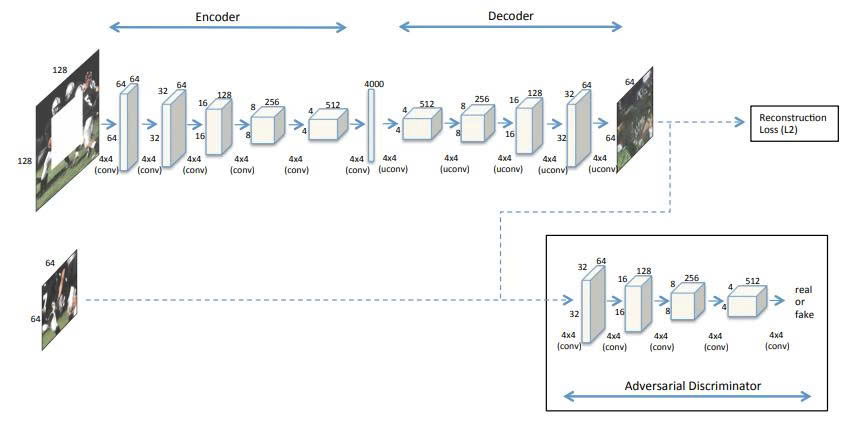
\includegraphics[width=1\linewidth]{context_encoder.jpg}
    \caption{Architecture of the Context Encoder framework. \textit{Adapted from}~\cite{pathak2016context}.}
    \label{fig:context_encoder}
\end{figure}

Figure~\ref{fig:context_encoder} presents the basic encoder--decoder formulation used by Context Encoders. The encoder compresses the visible image context into a latent representation, and the decoder predicts the missing region from this compact feature. This architecture is important historically because it shifted inpainting from hand-crafted patch search toward learned semantic completion. At the same time, the figure also reveals the limitation of early deep learning approaches: the missing region is restored through a relatively coarse bottleneck representation, which often leads to blurry outputs and weak fine-detail recovery in artistic or facial regions.

\medskip
\noindent\textbf{Global--Local Adversarial Inpainting.}

Iizuka et al.~\cite{iizuka2017global} proposed a globally and locally consistent image completion framework using two discriminators. The global discriminator enforces semantic coherence over the entire image, while the local discriminator focuses on texture realism within the inpainted region. Although effective, this approach increases training complexity and remains limited in modeling long-range dependencies.

\begin{figure}[H]
    \centering
    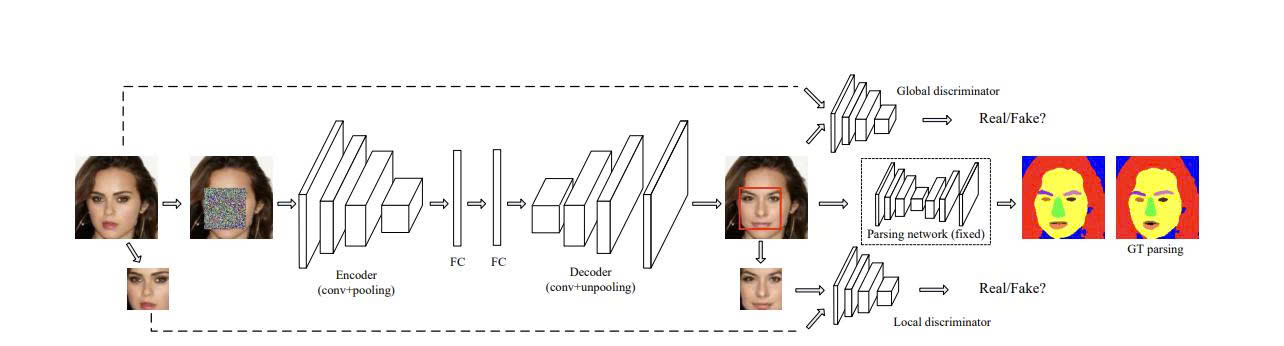
\includegraphics[width=1\linewidth]{global_local_inpainting.jpg}
    \caption{Global--local adversarial inpainting framework. \textit{Adapted from}~\cite{iizuka2017global}.}
    \label{fig:global_local}
\end{figure}

Figure~\ref{fig:global_local} illustrates the use of two adversarial objectives for image completion. The global discriminator evaluates whether the whole image is semantically coherent, while the local discriminator focuses more directly on the realism of the filled region. This design improves perceptual quality compared with purely pixel-wise reconstruction losses. For artwork restoration, however, the figure also highlights a challenge: local realism and global plausibility are not enough if the restored region changes painterly style or distorts face-specific structure.

\medskip
\noindent\textbf{Contextual Attention Inpainting.}

Yu et al.~\cite{yu2018contextual} introduced contextual attention, allowing features in missing regions to attend to distant patches in known areas. This mechanism improves texture reuse and reduces boundary artifacts. However, contextual attention increases computational cost and is primarily optimized for natural images rather than painterly textures.

\begin{figure}[H]
    \centering
    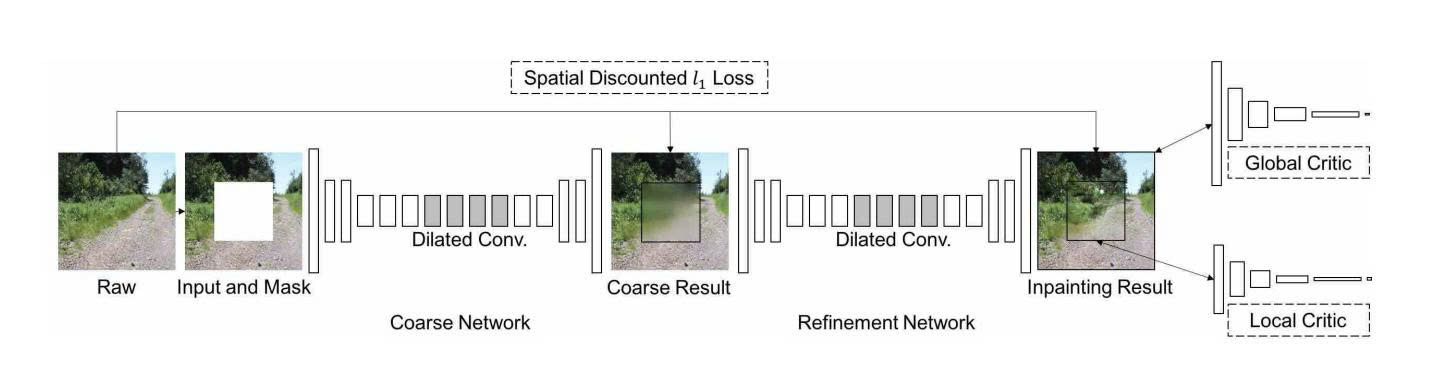
\includegraphics[
      width=1\linewidth,
      height=0.50\textheight,
      keepaspectratio
    ]{contextual_attention.jpg}
    \caption{Contextual attention framework for image inpainting. \textit{Adapted from}~\cite{yu2018contextual}.}
    \label{fig:contextual_attention}
\end{figure}

Figure~\ref{fig:contextual_attention} shows how contextual attention allows missing-region features to borrow information from spatially distant known regions. Instead of relying only on neighboring pixels, the model searches for semantically or texturally related patches elsewhere in the image and uses them to guide completion. This idea is relevant to artwork restoration because repeated brushstroke patterns or symmetric facial cues may appear outside the masked area. Nevertheless, contextual attention still depends on the availability of useful visible evidence, and it does not by itself guarantee accurate reconstruction when the mask removes most of the important facial structure.

\medskip
\noindent\textbf{Partial Convolution Inpainting.}

Liu et al.~\cite{liu2018partial} proposed partial convolutions, which condition convolution operations only on valid pixels and update the mask dynamically. This design improves robustness to irregular masks but still lacks global semantic reasoning.

\begin{figure}[H]
    \centering
    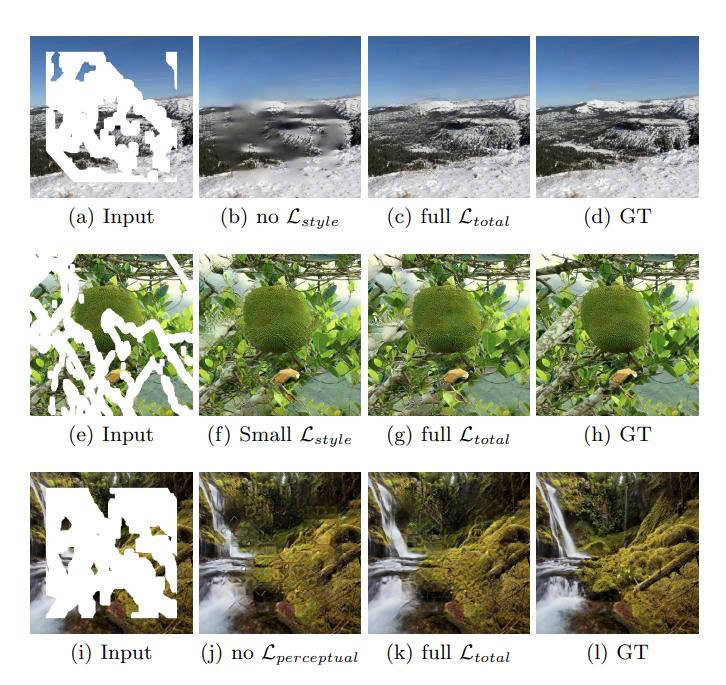
\includegraphics[width=0.5\linewidth]{partial_convolution.jpg}
    \caption{Partial convolution operation with dynamic mask updating. \textit{Adapted from}~\cite{liu2018partial}.}
    \label{fig:partial_conv}
\end{figure}

Figure~\ref{fig:partial_conv} illustrates the partial convolution mechanism. Unlike standard convolution, partial convolution computes feature responses only from valid pixels and updates the mask after each layer to indicate which locations have received sufficient contextual information. This is an important step toward handling irregular masks because the network becomes aware of which pixels are known and which are missing. However, the operation remains fundamentally local, so it cannot fully solve the long-range facial-structure reasoning required for large damaged regions in portrait artworks.

\medskip
\noindent\textbf{EdgeConnect: Structure-Guided Inpainting.}

Nazeri et al.~\cite{nazeri2019edgeconnect} introduced EdgeConnect, a two-stage framework that first predicts missing edges and then performs image completion guided by the predicted structure. This approach improves boundary sharpness but may be less reliable under abstract artistic styles.

\begin{figure}[H]
    \centering
    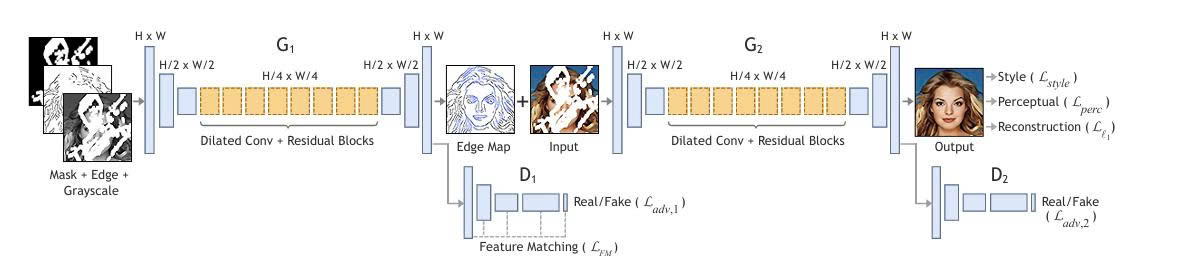
\includegraphics[width=1\linewidth]{edgeconnect.jpg}
    \caption{Two-stage structure-guided inpainting of EdgeConnect. \textit{Adapted from}~\cite{nazeri2019edgeconnect}.}
    \label{fig:edgeconnect}
\end{figure}

Figure~\ref{fig:edgeconnect} demonstrates a two-stage structure-guided inpainting strategy. The first stage predicts missing edges or contours, and the second stage uses those structural cues to synthesize the final image content. This separation is useful because it recognizes that plausible texture generation should be guided by an underlying structure. In the context of portrait artwork restoration, this idea is especially relevant for facial outlines and internal components; however, edge maps may become unreliable when artistic styles are soft, abstract, or when the mask removes too much of the original face.

\medskip
\noindent\textbf{Deep Image Prior.}

Ulyanov et al.~\cite{ulyanov2018dip} demonstrated that convolutional architectures themselves encode strong image priors. Deep Image Prior optimizes a randomly initialized CNN on a single image without training data. While conceptually insightful, it is computationally expensive and lacks semantic understanding.

\begin{figure}[H]
    \centering
    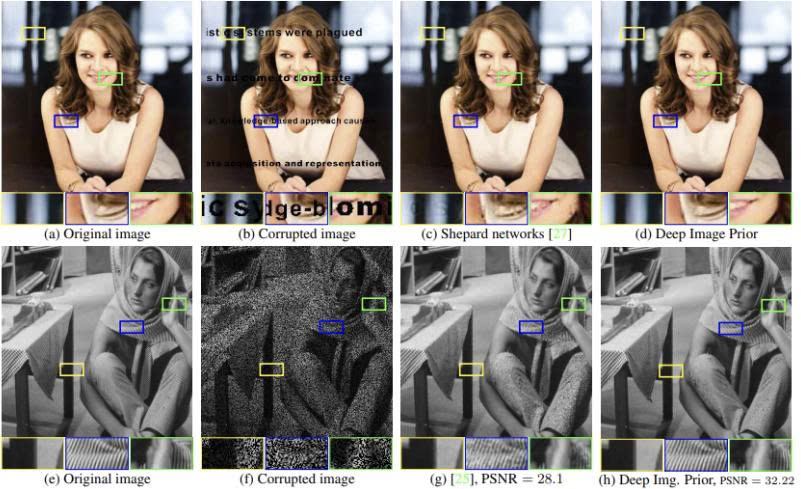
\includegraphics[width=0.75\linewidth]{deep_image_prior.jpg}
    \caption{Deep Image Prior for image inpainting. \textit{Adapted from}~\cite{ulyanov2018dip}.}
    \label{fig:dip}
\end{figure}

Figure~\ref{fig:dip} summarizes the Deep Image Prior concept, where a randomly initialized convolutional network is optimized directly on a single damaged image. The key observation is that the architecture of a CNN can act as an implicit image prior even without external training data. This is conceptually important for restoration because it shows that network structure itself can regularize reconstruction. However, for the thesis problem, this approach is less suitable as a main solution because it is slow, image-specific, and lacks learned semantic knowledge about portrait faces or painterly restoration patterns.

\section{Transformer-Based and Diffusion-Based Inpainting Methods}

Recent advances in image inpainting increasingly focus on global semantic reasoning and probabilistic generation to overcome the limitations of convolutional and GAN-based approaches. Transformer-based and diffusion-based models represent two complementary paradigms that dominate the state of the art. Transformer architectures introduce explicit long-range dependency modeling through self-attention, while diffusion models formulate inpainting as an iterative probabilistic denoising process capable of synthesizing high-fidelity textures under severe ambiguity.

\medskip
\noindent\textbf{ZITS: Transformer-Based Structure-Aware Inpainting.}

Zeng et al.~\cite{zeng2022zits} proposed ZITS (Zero-shot Image Inpainting with Transformer-based Structure), a transformer-based inpainting model designed to address large and irregular missing regions. ZITS decomposes the task into structure restoration and texture synthesis. The structure branch restores global structural cues, while the texture branch leverages Fourier-domain processing to synthesize high-frequency details. This design is relevant for artwork restoration where damage often disrupts contours and composition, although handcrafted structure--texture decomposition may limit flexibility across diverse artistic styles.

\begin{figure}[H]
    \centering
    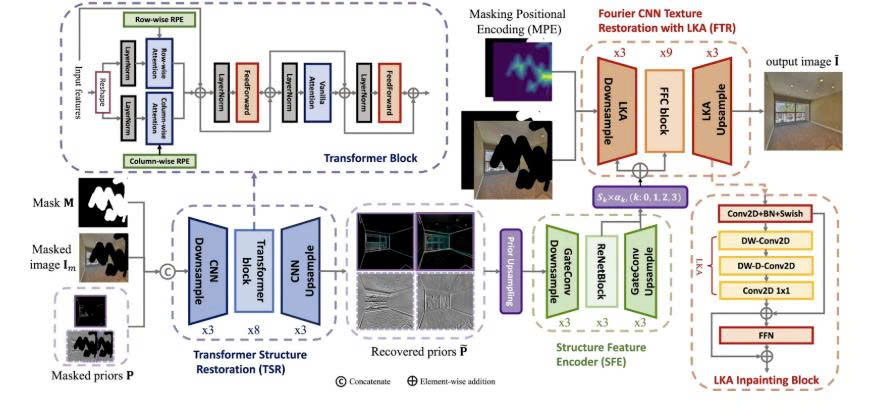
\includegraphics[width=1\linewidth]{zits.jpg}
    \caption{ZITS framework for zero-shot image inpainting. \textit{Adapted from}~\cite{zeng2022zits}.}
    \label{fig:zits}
\end{figure}

Figure~\ref{fig:zits} presents the ZITS framework, which separates inpainting into structure recovery and texture synthesis. The structural branch is designed to infer contours and layout, while the texture-related branch completes visual detail. This design is useful for large-hole inpainting because it explicitly acknowledges that structure and texture are different restoration problems. For this thesis, ZITS is relevant as a comparison method because portrait artwork restoration also requires both facial-layout recovery and painterly detail synthesis, although fixed structure--texture decomposition may not always adapt well to diverse painted faces.

\medskip
\noindent\textbf{ZITS++.}

ZITS++~\cite{zeng2023zitspp} extends ZITS with deeper transformer reasoning and improved interaction between structural and textural representations. It improves robustness under complex masks and diverse content, which can benefit artwork restoration by better preserving long-range stroke continuity and layout, at the cost of increased computation.

\begin{figure}[H]
    \centering
    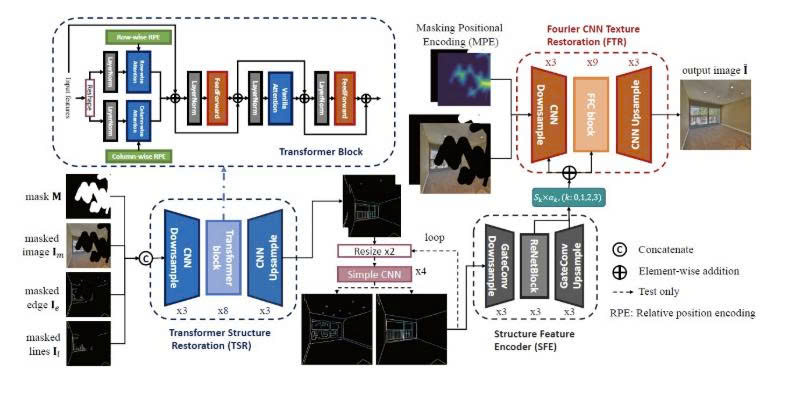
\includegraphics[width=1\linewidth]{zits_plus.jpg}
    \caption{ZITS++ enhanced transformer reasoning for inpainting. \textit{Adapted from}~\cite{zeng2023zitspp}.}
    \label{fig:zits_plus}
\end{figure}

Figure~\ref{fig:zits_plus} shows the enhanced reasoning design of ZITS++, which extends the original ZITS formulation with stronger transformer-based interactions between structure and texture representations. The figure is included to show the development trend from separate structure guidance toward deeper global reasoning. For artwork restoration, this is important because damaged portraits often require information to be propagated across distant facial and background regions. The limitation remains that increased reasoning capacity also increases complexity and does not necessarily guarantee faithful facial identity preservation.

\medskip
\noindent\textbf{Mask-Aware Transformer (MAT).}

Li et al.~\cite{li2022mat} introduced the Mask-Aware Transformer (MAT), a hybrid architecture combining convolutional feature extraction with transformer-based global reasoning. Its central innovation is mask-aware attention, which restricts self-attention to valid (unmasked) tokens and dynamically updates token validity during propagation. This design mitigates information leakage and stabilizes optimization under large-hole masks, making MAT a strong candidate for restoration scenarios where large paint loss and occlusions are common.

\begin{figure}[H]
    \centering
    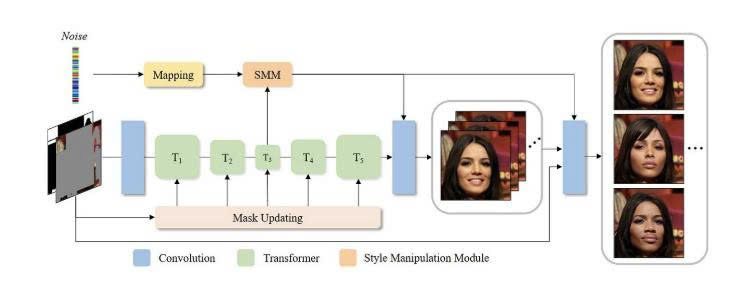
\includegraphics[width=1\linewidth]{mat_architecture.jpg}
    \caption{Mask-Aware Transformer (MAT) architecture for large-hole inpainting. \textit{Adapted from}~\cite{li2022mat}.}
    \label{fig:mat}
\end{figure}

Figure~\ref{fig:mat} illustrates the MAT architecture, which combines convolutional feature extraction, transformer reasoning, mask-aware attention, and style-modulated decoding. The figure is important for this thesis because MAT provides the technical foundation from which PARF is developed. Its mask-aware attention mechanism helps prevent invalid masked tokens from dominating self-attention, while dynamic mask propagation supports large-hole completion. However, the thesis does not claim MAT itself as the full contribution; instead, PARF builds on this foundation and adapts it toward portrait-artwork restoration through the framework choices described in Chapter~3.

\medskip
\noindent\textbf{Diffusion-Based Inpainting: RePaint.}

Lugmayr et al.~\cite{lugmayr2022repaint} proposed RePaint, adapting denoising diffusion probabilistic models for inpainting without retraining. Known pixels are repeatedly re-imposed during the denoising steps to preserve context, enabling high-quality synthesis even under challenging masks. This formulation established diffusion as a strong paradigm for inpainting because it can synthesize visually rich and perceptually convincing content under severe ambiguity. For artwork restoration, such behavior is attractive when damaged regions contain complex tone transitions or painterly textures. However, the repeated resampling strategy also makes RePaint computationally expensive, and its iterative reverse process is less convenient when both structural stability and practical inference efficiency are required.

\begin{figure}[H]
    \centering
    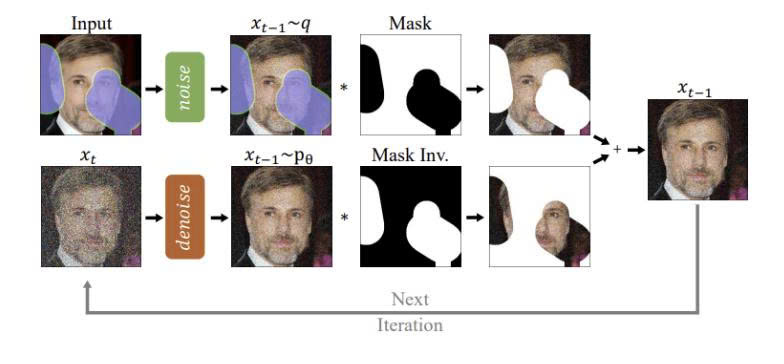
\includegraphics[width=1\linewidth]{repaint.jpg}
    \caption{RePaint: diffusion-based inpainting via conditional denoising. \textit{Adapted from}~\cite{lugmayr2022repaint}.}
    \label{fig:repaint}
\end{figure}

Figure~\ref{fig:repaint} visualizes the RePaint strategy, where known pixels are repeatedly enforced during the denoising process while the missing region is sampled through a diffusion model. This mechanism allows the method to generate perceptually rich completions under uncertain conditions. For artwork restoration, this is attractive because diffusion models can synthesize convincing local texture and tone transitions. The main limitation shown by the process is its iterative nature: repeated denoising and resampling can be computationally expensive and may still lack explicit control over exact facial structure.

\medskip
\noindent\textbf{Latent Diffusion and Structure-Guided Diffusion.}

Rombach et al.~\cite{rombach2022ldm} introduced latent diffusion models that operate in a compressed latent space to improve efficiency while maintaining high-quality synthesis. Inpainting can be achieved by conditioning the diffusion UNet on masked latent representations, typically using attention-based conditioning. This latent-space formulation significantly broadened the practical use of diffusion models for editing and inpainting, but the quality of the final restoration still depends strongly on how masked-image information is injected and how efficiently the reverse process is organized.

\begin{figure}[H]
    \centering
    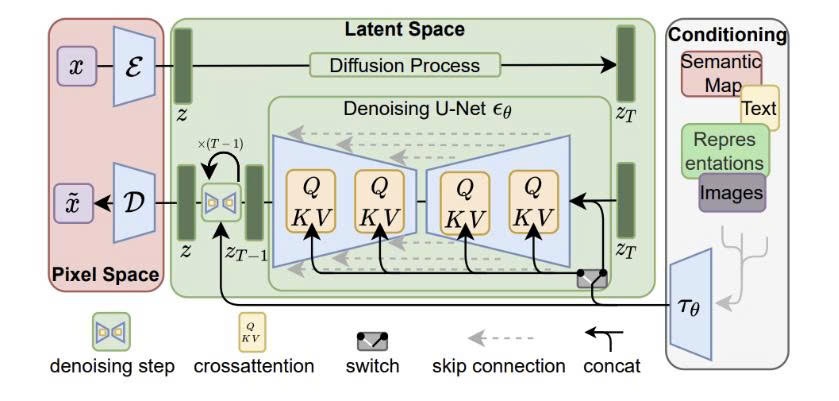
\includegraphics[width=1\linewidth]{latent.jpg}
    \caption{Latent diffusion framework for high-resolution image synthesis and inpainting. \textit{Adapted from}~\cite{rombach2022ldm}.}
    \label{fig:latent}
\end{figure}

Figure~\ref{fig:latent} illustrates the latent diffusion paradigm, in which images are encoded into a compressed latent space before the diffusion process is applied. This design reduces computational cost compared with pixel-space diffusion while preserving high-quality generative capability. In image inpainting, masked latent representations and conditioning information guide the model to regenerate missing content. For this thesis, latent diffusion is reviewed because it represents a major modern direction in generative restoration, although its output quality still depends heavily on how the mask and visible artwork context are injected into the denoising network.

\medskip
\noindent\textbf{BrushNet: Plug-and-Play Dual-Branch Diffusion.}

BrushNet~\cite{ju2024brushnet} is a recent ECCV 2024 diffusion-based inpainting model that improves conditioning quality through a decomposed dual-branch design. Instead of merging all signals into a single denoising stream, BrushNet separates noisy latent processing from masked-image feature injection and hierarchically introduces pixel-level masked-image features into a pre-trained diffusion backbone. The main strength of BrushNet is therefore stronger masked-region coherence and better utilization of visible-image context, while still preserving the plug-and-play flexibility of diffusion-based generation. This is relevant to artwork restoration because the surrounding painted region contains local style cues, tonal context, and texture evidence that should be injected explicitly rather than only through generic latent conditioning. At the same time, BrushNet still inherits the iterative cost of diffusion sampling and depends on a pre-trained diffusion backbone whose behavior is not explicitly optimized for the strict structural constraints of damaged portrait restoration. Importantly, the method is reproducible in practice because the authors provide an official paper, public repository, and released pretrained checkpoints for multiple settings~\cite{ju2024brushnet,brushnetrepo}.

\begin{figure}[H]
    \centering
    \IfFileExists{brushnet.jpg}{%
        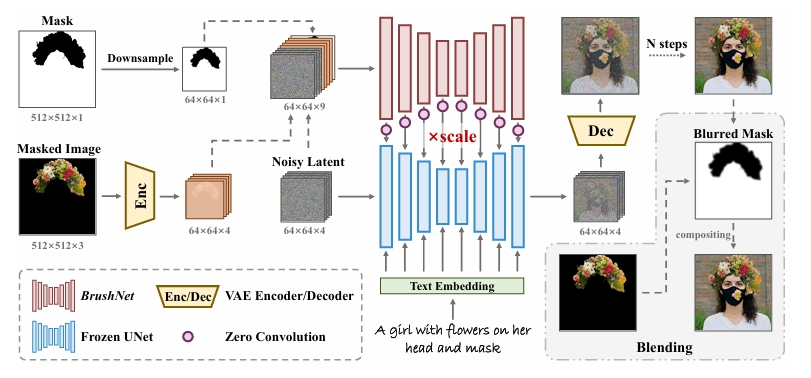
\includegraphics[width=1\linewidth]{brushnet.jpg}%
    }{%
        \IfFileExists{brushnet.jpg.jpeg}{%
            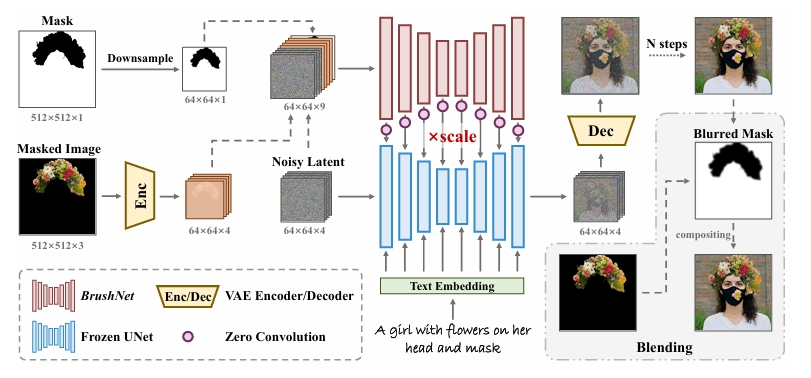
\includegraphics[width=1\linewidth]{brushnet.jpg.jpeg}%
        }{%
            \fbox{\parbox{0.88\linewidth}{\centering Placeholder for BrushNet framework figure\\Recommended filename: \texttt{brushnet.jpg}}}%
        }%
    }
    \caption{BrushNet: decomposed dual-branch diffusion with masked-image feature injection. \textit{Adapted from}~\cite{ju2024brushnet}.}
    \label{fig:brushnet}
\end{figure}

Figure~\ref{fig:brushnet} shows the central idea of BrushNet: separating the noisy latent denoising stream from the masked-image feature injection stream. The dual-branch design allows visible image information to be introduced more explicitly into the diffusion backbone, improving alignment between generated content and surrounding context. This is relevant to artwork restoration because local painterly cues around the damaged region should guide the completion rather than being ignored by a generic generative prior. The figure also clarifies why BrushNet is reviewed as a recent diffusion method: it improves conditioning quality, but still relies on diffusion sampling and a pre-trained generative backbone.

\medskip
\noindent\textbf{RAD: Region-Aware Diffusion for Efficient Inpainting.}

An even more recent direction is RAD (Region-Aware Diffusion)~\cite{kim2025rad}, reported as a CVPR 2025 diffusion-based inpainting method. RAD reformulates the inpainting process through a region-aware noise schedule, allowing masked and unmasked regions to evolve asynchronously while still preserving global image context within a simplified reverse process. Its main strength is efficiency: by avoiding more cumbersome conditioning loops, RAD substantially reduces inference time while maintaining strong inpainting quality. For artwork restoration, this region-aware formulation is appealing because damage often occupies only part of the canvas and should ideally be reconstructed without unnecessarily reprocessing already valid content. Nevertheless, although RAD improves practicality and speed, diffusion-based generation remains less directly constrained than structure-aware transformer reasoning when exact facial arrangement, contour continuity, or semantically sensitive portrait details must be preserved. The official paper and public code repository make RAD a reproducible recent reference for diffusion-based image inpainting research~\cite{kim2025rad,radrepo}.

\begin{figure}[H]
    \centering
    \IfFileExists{rad.jpg}{%
        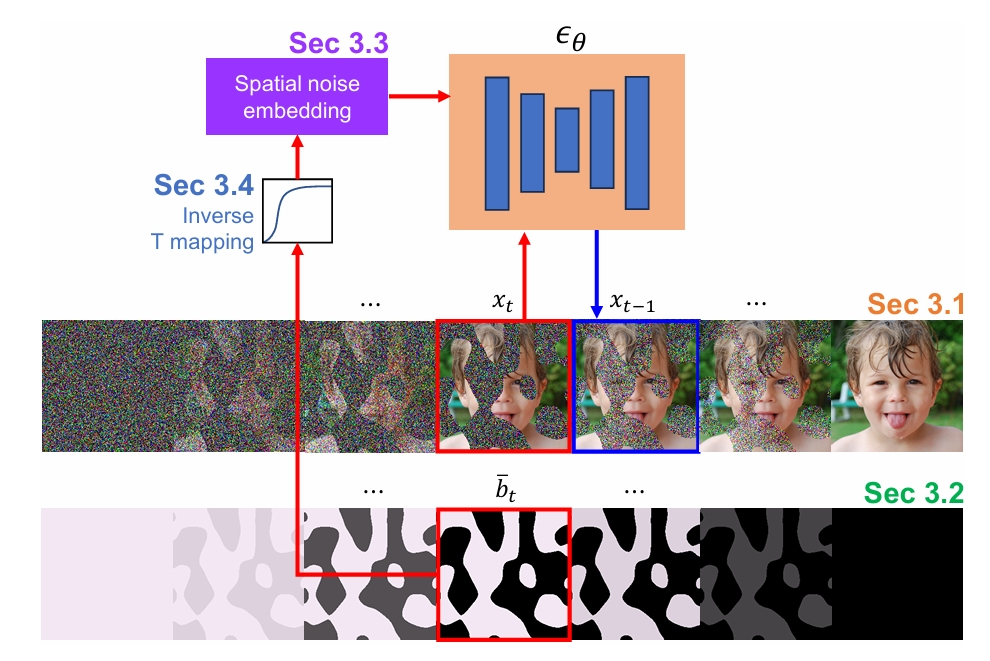
\includegraphics[width=1\linewidth]{rad.jpg}%
    }{%
        \IfFileExists{rad.jpg.jpeg}{%
            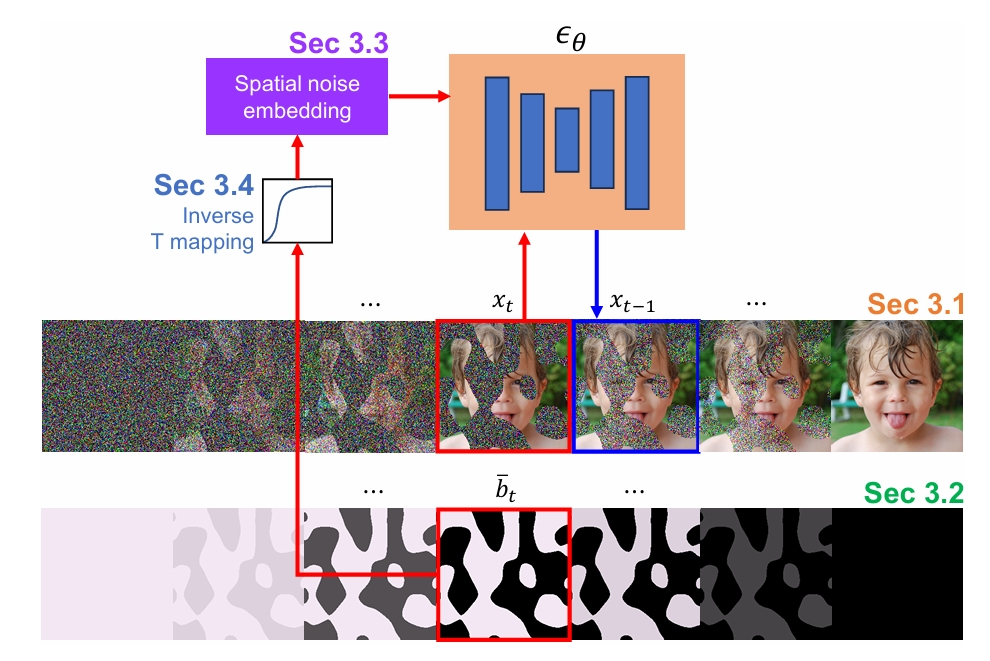
\includegraphics[width=1\linewidth]{rad.jpg.jpeg}%
        }{%
            \fbox{\parbox{0.88\linewidth}{\centering Placeholder for RAD framework figure\\Recommended filename: \texttt{rad.jpg}}}%
        }%
    }
    \caption{RAD: region-aware diffusion with simplified reverse scheduling for image inpainting. \textit{Adapted from}~\cite{kim2025rad}.}
    \label{fig:rad}
\end{figure}

Figure~\ref{fig:rad} illustrates RAD's region-aware diffusion formulation, where the masked and unmasked regions are handled with different noise schedules. This design aims to simplify the reverse process and reduce unnecessary computation on valid image regions. For artwork restoration, the idea is meaningful because damage usually affects only selected regions of the canvas, while the remaining content should be preserved. The figure is included to show the recent research trend toward efficient diffusion-based inpainting, although structural control over sensitive facial components remains a challenge compared with explicitly mask-aware transformer reasoning.

\medskip
\noindent\textbf{Commercial Image Editing Systems.}

Commercial foundation-model systems such as ChatGPT image editing and Gemini image editing show that large-scale generative editing has already moved into practical interactive use~\cite{openai_chatgpt_images,openai_chatgpt_editing,google_gemini_images,google_gemini_editing}. These platforms let users generate new images, upload existing ones, specify target regions, and request localized edits through natural-language instructions. This matters from an application perspective. It shows that image completion, object replacement, and conversational image editing are no longer limited to research prototypes.

For a literature review, these systems are worth mentioning because they illustrate the practical direction in which recent inpainting and image-editing research is moving. They show that modern generative pipelines can support conversational editing, region-based modification, instruction-guided refinement, and rapid visual iteration in a user-facing setting. This is relevant to artwork reconstruction because future restoration-support tools may no longer appear only as standalone research models. They may instead evolve into interactive systems in which conservators, researchers, or non-expert users guide restoration hypotheses through multimodal prompts.

At the same time, these commercial platforms are fundamentally different from academic methods such as ZITS, MAT, RePaint, BrushNet, and RAD. Their main strength lies in end-to-end usability, multimodal interaction, and broad generalization across tasks. Their value as scientific baselines is much more limited because they do not provide methodological transparency. The underlying architectures, model versions, training data mixtures, checkpoint selection procedures, internal editing constraints, and safety layers are not documented in a way that supports controlled replication. This lack of reproducibility matters in a thesis context, where comparisons must rest on stable model definitions, documented inference procedures, and evaluation settings that other researchers can inspect and repeat.

Therefore, ChatGPT and Gemini should be understood here as representative commercial applications rather than formal research baselines. They show that conversational and instruction-guided image editing has become a meaningful application domain. They also help situate restoration-oriented generative models within a broader technological landscape. However, because they do not provide the transparency required for rigorous experimental control, they are not included in Table~\ref{tab:trans_vs_diff} and are not used in the quantitative comparison later in Chapter~4.

\medskip
\noindent\textbf{Comparison Between Transformer and Diffusion Models.}

Transformer-based and diffusion-based methods address different parts of the inpainting problem. Transformers are strong at global structural reasoning and compositional coherence. Diffusion models are strong at probabilistic synthesis and texture realism. Within the diffusion family, the progression from RePaint to BrushNet and then to RAD also shows a broader trend. Early methods emphasized quality through iterative resampling. Later methods improved conditioning through more explicit masked-feature injection. Newer approaches increasingly target inference efficiency through simplified region-aware reverse processes. For artwork restoration, this distinction matters. Diffusion models are attractive when painterly texture and visually rich surface detail are important, but they still face tradeoffs in either structural consistency or computational cost. This helps explain why transformer-based models remain attractive when facial arrangement, contour continuity, and global composition must be preserved more explicitly.

\begin{table}[H]
\centering
\caption{Representative Modern Inpainting Methods Relevant to This Thesis}
\small
\begin{tabular}{|p{2.0cm}|p{1.6cm}|p{3.2cm}|p{3.0cm}|p{3.0cm}|}
\hline
\textbf{Method} & \textbf{Type} & \textbf{Core Idea} & \textbf{Strength} & \textbf{Limitation} \\
\hline
ZITS~\cite{zeng2022zits} & Transformer & Separates structure recovery from texture completion for large-hole inpainting & Strong global reasoning and contour recovery & Handcrafted structure splitting may reduce flexibility across diverse styles \\
\hline
ZITS++~\cite{zeng2023zitspp} & Transformer & Extends ZITS with deeper interaction between structure and texture streams & Better robustness under complex masks and stronger long-range reasoning & Higher computational cost \\
\hline
MAT~\cite{li2022mat} & Transformer & Uses mask-aware attention and dynamic validity propagation for large-hole completion & Strong global coherence and stable masked reasoning & Texture realism may still depend on task-specific adaptation \\
\hline
RePaint~\cite{lugmayr2022repaint} & Diffusion & Re-imposes known pixels during iterative denoising without retraining the base model & Strong perceptual realism and flexible completion & Slow inference due to repeated resampling \\
\hline
BrushNet~\cite{ju2024brushnet} & Diffusion & Plug-and-play dual-branch diffusion with masked-image feature injection & Better conditioning and coherent inpainting & Still inherits the cost of diffusion sampling \\
\hline
RAD~\cite{kim2025rad} & Diffusion & Region-aware diffusion with pixel-wise noise scheduling and a simplified reverse process & Faster inference with practical efficiency gains & Structural consistency in sensitive regions remains less direct than transformer reasoning \\
\hline
\end{tabular}
\normalsize
\label{tab:trans_vs_diff}
\end{table}

\section{Chapter Summary}

This chapter reviewed the development of image inpainting research and positioned the thesis within the broader technical landscape of digital artwork restoration. It began with classical PDE-based and exemplar-based methods, which rely on local smoothness, patch copying, and hand-crafted image priors~\cite{bertalmio2000inpainting,criminisi2004exemplar,barnes2009patchmatch}. These methods remain historically important because they established the basic idea of filling missing regions from surrounding context. Their limitations become clear, however, when the missing area is large, semantically important, or strongly textured. In portrait artwork restoration, local propagation or patch copying is usually not enough because the model must reconstruct facial structure, preserve painterly continuity, and avoid visible distortions around the eyes, nose, mouth, and facial contour.

The chapter then examined the shift from hand-crafted restoration to learned inpainting. CNN and GAN methods introduced learned visual priors and improved the perceptual realism of restored images~\cite{pathak2016context,iizuka2017global}. These approaches are important because they allow the model to learn plausible visual content from training data rather than relying only on local image continuity. Nevertheless, convolutional architectures often remain limited in their ability to model long-range relationships, which can lead to structural inconsistencies in complex scenes. This limitation is especially relevant for portrait artwork reconstruction, where the relative arrangement of facial components must remain coherent across the whole damaged region.

Modern transformer-based approaches address part of this problem by improving global reasoning and long-range dependency modeling. Methods such as ZITS, ZITS++, and MAT demonstrate that transformer mechanisms can support large-hole completion, structure-texture reasoning, and mask-aware validity propagation~\cite{zeng2022zits,zeng2023zitspp,li2022mat}. These studies are directly relevant to the thesis because portrait artwork restoration requires stable facial layout estimation before local detail can be refined. At the same time, the review also showed that a strong baseline architecture alone is not always sufficient for the specific demands of portrait artwork reconstruction. This motivates the thesis direction of adapting and extending a transformer-based foundation into PARF, a framework focused more explicitly on damaged painted portraits.

The diffusion-based literature was also reviewed because diffusion models have become increasingly important in recent image inpainting research. RePaint represents an early diffusion-based inpainting method that achieves strong perceptual realism through iterative resampling~\cite{lugmayr2022repaint}, while latent diffusion models provide a more scalable generative foundation~\cite{rombach2022ldm}. More recent methods such as BrushNet and RAD show how the field is moving toward better conditioning and more efficient inference~\cite{ju2024brushnet,kim2025rad}. BrushNet improves diffusion inpainting by injecting masked-image features through a dual-branch design, whereas RAD improves practicality through region-aware noise scheduling and a simplified reverse process. These developments show that diffusion methods are powerful for texture realism and generative quality, but they may still face challenges in computational efficiency and precise structural control for semantically sensitive portrait regions.

Finally, the chapter discussed commercial image-editing systems such as ChatGPT image editing and Gemini image editing as examples of how generative image editing has entered practical application contexts~\cite{openai_chatgpt_images,openai_chatgpt_editing,google_gemini_images,google_gemini_editing}. These systems are useful for understanding the broader direction of interactive visual editing, but they are not appropriate as scientific baselines because their architectures, model versions, training data, and inference procedures are not fully transparent or reproducible. Therefore, the thesis grounds its technical comparison in academic methods with documented mechanisms and reproducible resources. Overall, Chapter~2 establishes the research motivation for PARF: existing methods have made substantial progress in inpainting, but portrait artwork reconstruction still requires a framework that balances global facial structure, local painterly refinement, and transparent evaluation. This motivation leads directly to the methodology presented in Chapter~3.



% ============================================================
% Chapter 3: Methodology
% ============================================================
\chapter{Methodology}

\section{Framework Overview}

This chapter presents the methodological design of the Portrait Artwork Reconstruction Framework (PARF) for portrait artwork reconstruction. PARF is developed on top of a strong mask-aware transformer inpainting foundation~\cite{li2022mat}, and is reformulated here as a portrait-artwork-oriented restoration pipeline. The methodological contribution of this thesis is therefore the design of a complete PARF pipeline that adapts this foundation, adds portrait-oriented deep-stage adaptation, introduces a dedicated refinement stage, and couples the architecture with style guidance and frequency-aware training. The chapter first introduces the overall framework, then focuses on the major architectural components and the training objective used to optimize the model. Experimental data preparation, results, and evaluation are deferred to Chapter~4.

\clearpage
\begin{figure}[p]
    \centering
    \IfFileExists{fig3_1_framework_overview.png}{%
        \includegraphics[width=\linewidth,height=0.90\textheight,keepaspectratio]{fig3_1_framework_overview.png}%
    }{%
        \IfFileExists{fig3_1_framework_overview.png.png}{%
            \includegraphics[width=\linewidth,height=0.90\textheight,keepaspectratio]{fig3_1_framework_overview.png.png}%
        }{%
            \fbox{\parbox{0.92\linewidth}{\centering Placeholder for Figure 3.1\\Overall framework overview of PARF for face artwork restoration.}}%
        }%
    }
    \caption{Overall architecture of PARF for portrait artwork reconstruction.}
    \label{fig:framework_overview}
\end{figure}
\clearpage

As illustrated in Figure~\ref{fig:framework_overview}, PARF follows a coarse-to-refinement restoration pipeline designed specifically for portrait artwork reconstruction.
The input of the framework consists of a masked FACEART image and its corresponding binary mask.
The masked image provides the visible artistic context, while the binary mask explicitly identifies the corrupted region that must be reconstructed.
These two inputs are first passed through a convolutional front-end, denoted as \texttt{conv\_first}, which converts the image and mask information into an initial feature representation suitable for transformer reasoning.
This early convolutional step is important because it preserves local color transitions, edge cues, and brushstroke-related visual evidence before the features are processed at deeper semantic levels.

The first major component of PARF is Stage~1, an encoder--decoder transformer module responsible for coarse structural restoration.
This stage contains five transformer stages, denoted as T1--T5, organized in a multi-scale progression.
The early and late transformer stages operate at relatively higher spatial resolution, while the middle bottleneck stage operates at $16\times16$ resolution, where global semantic reasoning is concentrated.
In the thesis design, the first phase introduces relative position bias and mask-aware additive bias across the transformer path, while the later phase strengthens the deeper stages using residual adapters at the $32\times32$ and $16\times16$ resolutions.
These additions are intended to make the transformer backbone more suitable for portrait artwork restoration, where the model must infer missing facial components from sparse surrounding context without losing global facial proportion.

The mask-updating path shown inside Stage~1 represents the mechanism by which valid contextual information is progressively propagated into the corrupted region.
Rather than treating the original binary mask as a fixed constraint throughout the network, PARF updates the effective validity information as the transformer stages infer more reliable content.
This is particularly useful for large-hole portrait restoration because the missing region may cover semantically connected facial parts such as the eyes, nose, mouth, or facial contour.
The output of Stage~1 is therefore a coarse restored image that establishes the main facial layout and provides a structurally plausible intermediate result.

The right side of Figure~\ref{fig:framework_overview} illustrates the style-conditioning branch.
A latent noise vector is passed through a mapping network and then into the Style Manipulation Module (SMM), which produces style-related modulation information for the reconstruction process.
In PARF, this branch supports painterly consistency by guiding the restored region toward the color distribution, texture statistics, and visual style of the surrounding artwork.
This is important because portrait artwork reconstruction requires more than semantic face completion: the restored region must also blend with the original painting style rather than appearing as a generic natural-image face.

Stage~2 performs refinement on top of the Stage~1 coarse output.
Its input combines the coarse result, the visible known pixels, and the binary mask, allowing the refinement network to focus on improving the generated region while preserving the unmasked content.
The Stage~2 refinement encoder compresses the intermediate result into a compact representation, and the $16\times16$ style bottleneck uses deterministic latent gating to combine structural features with style-conditioned guidance.
The final style-conditioned decoder then produces the restored FACEART image with improved local facial coherence, smoother boundary transition, and stronger painterly continuity.

The optimization block at the bottom of the framework summarizes the training objectives used to guide PARF.
Adversarial loss encourages visually realistic restoration, perceptual loss supports semantic and feature-level similarity, and stabilized Focal Frequency Loss emphasizes hard-to-reconstruct frequency components that are important for painterly detail and facial texture.
Together, these losses support the thesis objective of improving both structural plausibility and visual quality in restored portrait artworks.

This organization is motivated by the requirements of portrait artwork reconstruction, where large corrupted regions must first be restored at the structural level before fine visual detail can be improved.
As a result, PARF combines global contextual reasoning, style-conditioned restoration, deterministic latent guidance, and frequency-aware optimization into a single portrait-oriented artwork reconstruction framework.

From a methodological perspective, PARF should be understood as a thesis-specific reconstruction framework built from an established transformer inpainting foundation~\cite{li2022mat}. The contribution is the way this foundation is reorganized, extended, and trained for portrait artwork reconstruction. The concrete differences from the baseline are the portrait-artwork restoration framing, the deep-stage residual adapter enhancement, the deterministic latent-guidance integration, the explicit two-stage refinement emphasis, and the frequency-domain training design introduced to improve painterly detail reconstruction. Thus, Figure~\ref{fig:framework_overview} should be read as the overall PARF design: the citation identifies the technical source, while the contribution is the thesis-specific arrangement of modules and objectives around the portrait-artwork restoration problem.

% ------------------------------------------------------------
% ------------------------------------------------------------
\section{Stage 1 Coarse Restoration}

The first stage of PARF performs coarse reconstruction of the damaged artwork image. Its role is to recover the global structure of the missing region before fine-grained refinement is applied, which is especially important for reconstructing the rough facial layout in portrait artworks. In terms of design origin, this stage is developed in the thesis on top of a convolution-first and transformer-based reasoning backbone~\cite{li2022mat}, but it is formulated here as the front-end of a portrait-artwork reconstruction pipeline rather than as a direct restatement of the baseline. Operationally, Stage~1 first encodes the masked artwork into compact features, then performs global reasoning across valid regions, and finally decodes a coarse prediction for the unknown area. The benefit of this phase is that it establishes a structurally plausible estimate that later allows Stage~2 to concentrate on local detail recovery instead of re-solving global completion from scratch.

% ------------------------------------------------------------
\vspace{0.35\baselineskip}
\noindent\textbf{Convolutional Head for Artwork Restoration.}\par

Within PARF, the convolutional head serves as the front-end feature extractor. It prepares the masked artwork for transformer reasoning. This component follows a convolution-first inpainting design~\cite{li2022mat}, but in the thesis it is integrated into the proposed restoration pipeline and tailored to artwork-conditioned inputs. Its role is to encode visible content together with mask information into compact local features before the transformer stages perform global reasoning. The practical benefit is that early artistic cues, such as color transitions, brushstroke orientation, and local edge continuity, are preserved while the spatial resolution is reduced efficiently.
In the thesis presentation, this front-end is treated as a thesis-developed entry component because its role, input composition, and downstream coupling are defined by the proposed portrait-artwork pipeline rather than by the baseline alone. This framing matters because the quality of the initial local encoding affects how reliably later stages reconstruct facial layout and painterly texture continuity.

In PARF, the first-stage input feature is formulated by concatenating the centered binary mask with the visible image content:
\begin{equation}
\mathbf{F}_{\mathrm{in}} = \mathrm{Concat}\big(\mathbf{M} - 0.5,\; \mathbf{I} \odot \mathbf{M}\big),
\end{equation}
where $\mathbf{I}$ denotes the input artwork image, $\mathbf{M}$ is the binary mask, and $\odot$ denotes element-wise multiplication. This representation preserves known pixels while explicitly informing the network of missing regions, which makes the subsequent transformer reasoning more aware of where contextual completion is required.

% ------------------------------------------------------------
\vspace{0.35\baselineskip}
\noindent\textbf{Initial Coarse Reconstruction Strategy.}\par

After feature extraction and transformer reasoning, the first stage generates a coarse reconstruction of the missing content. The role of this strategy in the thesis is to recover global arrangement and facial structure rather than to directly synthesize the final high-frequency result. This part is implemented as a thesis-level coarse-to-refinement design choice built upon the cited transformer reasoning backbone~\cite{li2022mat}, and it is formulated so that Stage~1 predicts the unknown content while the visible pixels remain fixed.

In the proposed reconstruction formulation, the decoded Stage~1 prediction is ensembled with the visible input pixels as
\begin{equation}
\hat{\mathbf{I}}^{(1)} = \hat{\mathbf{I}}_{\mathrm{raw}}^{(1)} \odot (1-\mathbf{M}) + \mathbf{I} \odot \mathbf{M},
\end{equation}
where $\hat{\mathbf{I}}_{\mathrm{raw}}^{(1)}$ denotes the raw decoder output before visible-pixel reinsertion. This formulation ensures that the first stage concentrates on reconstructing only the missing regions while preserving known content. The benefit is that large and semantically important portrait regions can be completed in a stable coarse manner first, which provides a much stronger starting point for later refinement of facial details and painterly textures.

\begin{figure}[H]
    \centering
    \IfFileExists{fig3_4_stage1_coarse_restoration.png}{%
        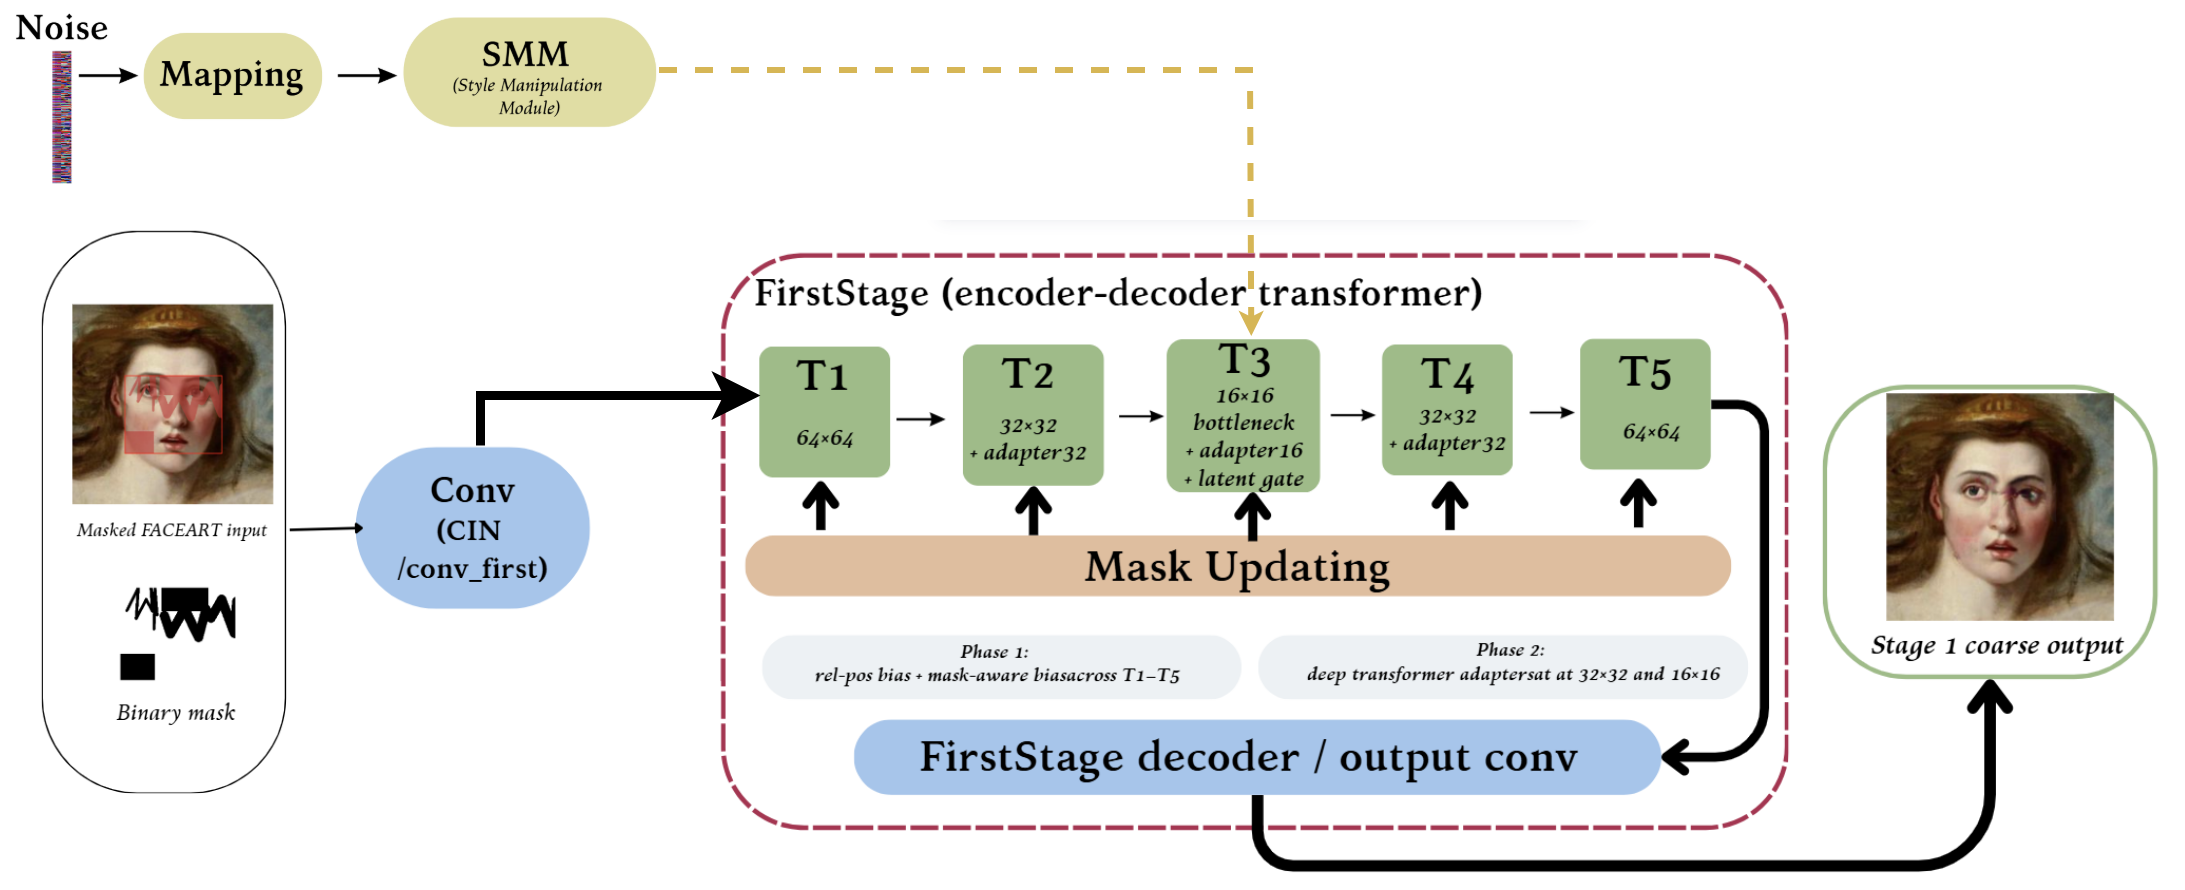
\includegraphics[width=0.95\linewidth]{fig3_4_stage1_coarse_restoration.png}%
    }{%
        \fbox{\parbox{0.85\linewidth}{\centering Placeholder for Figure 3.4\\Illustration of the Stage 1 coarse restoration process.}}%
    }
    \caption{Illustration of the Stage~1 coarse restoration process.}
    \label{fig:stage1_coarse_restoration}
\end{figure}

Figure~\ref{fig:stage1_coarse_restoration} illustrates the role of Stage~1 as the coarse reconstruction stage of PARF. The figure shows that the masked artwork and binary mask are first encoded into features, then processed through the transformer reasoning path, and finally decoded into an initial completed image. The main purpose of this stage is not to generate the final high-detail restoration, but to recover the global facial layout and establish a plausible structural foundation. This coarse result is especially important for portrait artwork because later refinement can only improve local details effectively if the main facial arrangement has already been reconstructed in a stable way.

The contribution represented by Figure~\ref{fig:stage1_coarse_restoration} should therefore be understood at the framework-adaptation level rather than as a claim that the entire transformer backbone is invented from scratch. Compared with a general large-hole inpainting baseline~\cite{li2022mat}, PARF reformulates the first stage as a portrait-artwork-oriented coarse restoration module. The difference is visible in four specific points. First, the input is explicitly framed as a masked FACEART portrait image together with a binary mask, so the restoration target is tied to face-sensitive artwork damage rather than generic image completion. Second, the convolutional front-end is used as an artwork-conditioned entry component that preserves local painterly evidence before global reasoning. Third, the transformer path is interpreted and extended for portrait structure recovery, with the deeper $32\times32$ and $16\times16$ reasoning stages serving as the locations for thesis-specific residual adaptation. Fourth, the output of Stage~1 is intentionally treated as a coarse structural prior for Stage~2 instead of being considered the final restoration result. In this sense, Figure~\ref{fig:stage1_coarse_restoration} provides the overview of PARF's first contribution: adapting a strong transformer inpainting foundation into a controlled coarse-restoration stage for damaged portrait artworks.

This distinction from the baseline is important for the thesis argument. Existing large-hole transformer inpainting already provides mask-aware reasoning and dynamic validity propagation~\cite{li2022mat}, but it does not by itself define the two-stage portrait-artwork workflow used in this study. PARF's contribution at this point is to reorganize the baseline reasoning capability into a task-specific Stage~1 whose goal is stable facial layout recovery, preservation of visible artwork pixels, and preparation of a structurally reliable intermediate result for later refinement. Therefore, the figure should be read as the methodological overview of how the cited inpainting backbone is repurposed and extended for the thesis problem.

% ------------------------------------------------------------
\section{Transformer Body}

The transformer body is the central reasoning component of PARF. It is responsible for modeling long-range dependencies between visible regions and missing areas, enabling the reconstruction process to infer semantically plausible content under large and irregular masks. At the architectural level, this reasoning backbone is developed from a prior mask-aware transformer design~\cite{li2022mat}, but in this thesis it is extended and integrated as part of a portrait-artwork-oriented restoration system.

In PARF, the first-stage transformer path is composed of five sequential reasoning stages with depths $[2,3,4,3,2]$. Their spatial progression follows a symmetric multi-scale pattern, moving from $64\times64$ features to $32\times32$, then to a $16\times16$ bottleneck, and finally expanding back through $32\times32$ and $64\times64$ representations. This organization compresses the representation toward a bottleneck for global reasoning and then expands it again for reconstruction. The deeper $32\times32$ and $16\times16$ stages are also the locations where the thesis places stronger task-specific adaptation.

% ------------------------------------------------------------
\subsection{Transformer Reasoning in PARF}

In PARF, the transformer body is responsible for global reasoning across visible and missing regions, which is essential when portrait structures are interrupted by large holes. This reasoning module is developed from a prior mask-aware transformer formulation~\cite{li2022mat}, but it is presented here as part of the thesis-developed restoration system and as the basis onto which the later adapter enhancement is introduced. Mechanistically, the transformer path uses adjusted block updates and contextual attention to propagate information through valid tokens while progressively refining the hidden representation. The benefit is that the framework can model long-range facial relationships and compositional consistency more effectively than a purely local convolutional pipeline.

To improve optimization stability in large-hole reconstruction, PARF employs an adjusted transformer block rather than a standard transformer design~\cite{li2022mat}. In the thesis pipeline, its role is to stabilize feature propagation when a substantial proportion of tokens correspond to invalid or masked regions.

\begin{equation}
\mathbf{X}'_{k,\ell} = \mathrm{FC}\big([\mathrm{MCA}(\mathbf{X}_{k,\ell-1}),\; \mathbf{X}_{k,\ell-1}]\big),
\end{equation}
\begin{equation}
\mathbf{X}_{k,\ell} = \mathrm{MLP}(\mathbf{X}'_{k,\ell}),
\end{equation}
where $\mathbf{X}_{k,\ell}$ denotes the output of the $\ell$-th block in the $k$-th stage. In this formulation, contextual reasoning and feature update are separated in a way that avoids overly aggressive residual accumulation over masked regions, which is beneficial for stable artwork reconstruction.

\begin{figure}[H]
    \centering
    \IfFileExists{fig3_5_transformer_stage.jpg}{%
        \includegraphics[width=0.9\linewidth]{fig3_5_transformer_stage.jpg}%
    }{%
        \IfFileExists{mat_transformer_stage.jpg}{%
            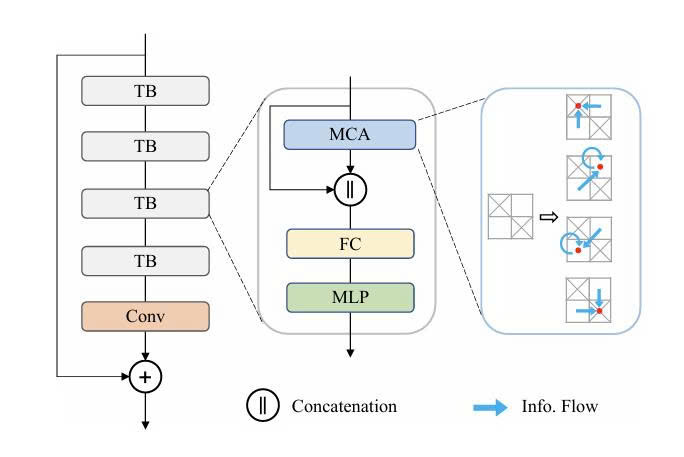
\includegraphics[width=0.9\linewidth]{mat_transformer_stage.jpg}%
        }{%
            \fbox{\parbox{0.82\linewidth}{\centering Placeholder for Figure 3.5\\Structure of the transformer stage used in PARF.}}%
        }%
    }
    \caption{Structure of the transformer stage used in PARF.}
    \label{fig:transformer_stage}
\end{figure}

Figure~\ref{fig:transformer_stage} explains the internal transformer stage used for global contextual reasoning in PARF~\cite{li2022mat}. The figure highlights how token features are processed through contextual attention and subsequent feature transformation so that information from valid visible regions can influence the masked region. This is different from a purely convolutional operation because the transformer stage can model long-range relationships across distant parts of the artwork. For portrait restoration, this is essential because the missing eye, nose, or mouth region may need to be inferred from global facial symmetry, head orientation, and surrounding painterly context rather than from immediate local pixels alone. The contribution represented here is the role assigned to this reasoning stage inside PARF: it becomes the structural reasoning core for portrait-artwork restoration, while the thesis adds portrait-specific deep-stage adaptation and a later refinement stage around it.

% ------------------------------------------------------------
\vspace{0.35\baselineskip}
\noindent\textbf{Multi-Head Contextual Attention.}\par

The transformer body applies multi-head contextual attention to model long-range interactions between valid tokens and masked regions~\cite{li2022mat}. Its role in PARF is to borrow information from distant but semantically relevant visible areas. The operation is expressed through mask-aware attention, where query-key interactions are modulated by an additive bias that suppresses invalid tokens. The main benefit is that restoration does not depend only on local neighborhoods, which helps preserve global facial symmetry, contour continuity, and coherence across separated visible regions.
Within PARF, the contribution is the integration and extension context of this attention mechanism rather than the original attention formula itself. Specifically, the mask-aware reasoning path is embedded into a portrait-artwork reconstruction pipeline together with deep-stage residual adapters, deterministic latent guidance, and the Stage~2 refinement module. This integration is particularly beneficial when missing facial regions must be inferred from sparse but semantically meaningful visible evidence distributed across the artwork.

Following the mask-aware attention formulation~\cite{li2022mat}, the attention operation can be written as:
\begin{equation}
\mathrm{Att}(\mathbf{Q}, \mathbf{K}, \mathbf{V}) =
\mathrm{Softmax}\left(\frac{\mathbf{Q}\mathbf{K}^T + \mathbf{M}'}{\sqrt{d_k}}\right)\mathbf{V},
\end{equation}
where $\mathbf{Q}$, $\mathbf{K}$, and $\mathbf{V}$ are the query, key, and value matrices, respectively. In the mask-aware formulation used by PARF, the additive attention bias $\mathbf{M}'$ is defined element-wise as
\begin{equation}
\mathbf{M}'_{ij} =
\begin{cases}
0, & \text{if token } j \text{ is valid},\\
-\tau, & \text{if token } j \text{ is invalid},
\end{cases}
\end{equation}
where $\tau$ is a large positive constant used to suppress attention to invalid tokens.

% ------------------------------------------------------------
\subsection{Residual Adapter Enhancement}

The thesis extends the transformer body with residual adapters inserted into the deeper transformer stages. The general idea of lightweight adapter-based specialization is related to parameter-efficient adaptation strategies in deep networks~\cite{houlsby2019parameter}, while the specific placement and use of adapters at the $32\times32$ and $16\times16$ transformer stages are thesis-developed design choices within PARF. The role of this component is to provide task-specific adaptation capacity in compact high-semantic feature spaces without replacing the backbone reasoning path. Unlike the cited baseline architecture~\cite{li2022mat}, this module is selectively enabled only in the deeper reasoning stages. The benefit of this design is that portrait-artwork-specific adaptation is concentrated where the representation is semantically strongest, allowing the model to better specialize to damaged facial structures while preserving the overall efficiency of the backbone.

In practical terms, the residual-adaptation idea is used to add lightweight task-specific capacity to the deeper transformer path without replacing the backbone reasoning mechanism. The added branch first transforms the deep token features through a compact projection pathway and then feeds the result back into the main representation with a controlled residual effect. This design keeps the added specialization lightweight at the beginning of training while still allowing the model to devote more capacity to portrait-artwork-specific structure recovery in deeper semantic stages. For PARF, the importance of this component is not a new generic adapter formula, but the decision to concentrate portrait-specific adaptation in the deep transformer layers where large-hole facial reasoning is most sensitive.

% ------------------------------------------------------------
\vspace{0.35\baselineskip}
\noindent\textbf{Dynamic Mask Updating.}\par

A key characteristic of the transformer reasoning path is the dynamic updating of the validity mask during propagation~\cite{li2022mat}. In PARF, the role of this mechanism is to expand the effective known region as reliable contextual information is inferred. Instead of keeping the original binary mask fixed throughout the network, the model progressively updates valid-token regions as information is propagated through attention. The benefit is that contextual evidence can move gradually into corrupted facial areas, which is especially useful when reconstructing semantically coordinated regions such as the eyes, nose, and mouth.
The thesis contribution is the way this validity propagation is placed inside a portrait-oriented Stage~1 coarse restoration module and connected to the later Stage~2 refinement input. This makes the mechanism especially valuable for portrait artwork reconstruction, where a gradual expansion of valid context can stabilize completion over large facial holes.

\begin{figure}[H]
    \centering
    \IfFileExists{fig3_6_mask_updating.jpg}{%
        \includegraphics[width=0.75\linewidth]{fig3_6_mask_updating.jpg}%
    }{%
        \IfFileExists{mat_mask_update.jpg}{%
            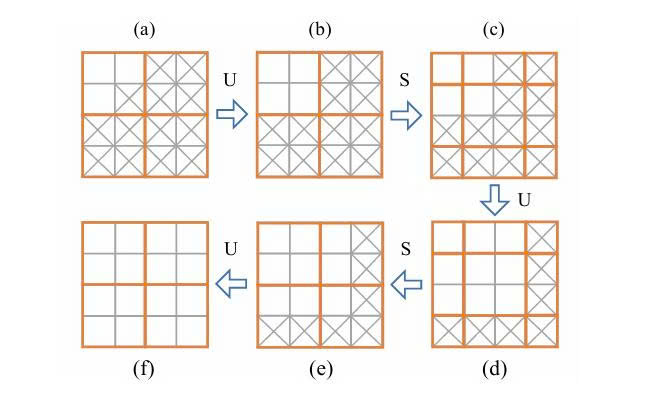
\includegraphics[width=0.75\linewidth]{mat_mask_update.jpg}%
        }{%
            \fbox{\parbox{0.72\linewidth}{\centering Placeholder for Figure 3.6\\Illustration of the dynamic mask updating strategy during transformer reasoning.}}%
        }%
    }
    \caption{Illustration of the dynamic mask updating strategy during transformer reasoning.}
    \label{fig:mask_updating}
\end{figure}

Figure~\ref{fig:mask_updating} illustrates how the validity mask evolves during transformer reasoning~\cite{li2022mat}. PARF uses this mechanism as part of the Stage~1 portrait-structure recovery process. At the beginning, only the originally visible regions are treated as reliable context, while the masked region is considered invalid or unknown. As attention propagates information through the feature map, the effective valid area is gradually expanded, allowing newly inferred regions to participate in later reasoning steps. This process is important for large-hole portrait restoration because the model cannot fill the entire face region in one local operation; instead, it must progressively propagate evidence from reliable visible pixels into the missing facial area. Compared with the baseline presentation, the contribution in PARF is that the updated validity information is used to produce a coarse structural prior that is explicitly passed to Stage~2 refinement rather than being treated only as part of a single-stage completion path.

% ------------------------------------------------------------
\section{Style Conditioning and Latent Guidance}

Artwork reconstruction requires not only structural plausibility but also consistency with artistic style. For this reason, PARF incorporates style conditioning and latent guidance mechanisms whose role is to align the reconstructed region with the visible artistic context. The style-manipulation pathway follows a prior style-modulated inpainting design~\cite{li2022mat}, while the deterministic latent-guidance integration is treated in the thesis as part of the proposed PARF design. Mechanistically, the framework first forms a style representation and then blends it with feature tokens through a deterministic gate before decoding. The benefit is that the restored facial region can better preserve color tone, texture statistics, and painterly continuity rather than being reconstructed only from structure-oriented cues.

In the style-manipulation formulation used as the starting point~\cite{li2022mat}, a latent-noise pathway is first transformed into an unconditional style signal and then combined with image-conditioned features to form a style code for decoding. In the original style-modulated design, this code influences the decoder so that reconstruction is not guided only by structure, but also by stylistic cues derived from the latent branch and the visible image context. For the thesis discussion, the important point is not the full algebra of the original modulation process, but the fact that PARF inherits a style-guidance pathway and then reuses it in a more task-specific way for portrait-artwork refinement.

In the proposed style-guidance design, style-related latent information is further integrated through a deterministic latent gate. Given feature tokens $\mathbf{f}$ and latent guidance $\mathbf{l}$, the gate is computed as
\begin{equation}
\mathbf{g} = \sigma\big(f_{\theta}([\mathbf{f}, \mathbf{l}])\big),
\end{equation}
and the blended representation becomes
\begin{equation}
\tilde{\mathbf{f}} = \mathbf{g} \odot \mathbf{f} + (1-\mathbf{g}) \odot \mathbf{l}.
\end{equation}
This mechanism enables PARF to adaptively balance structural features and latent style guidance rather than relying on a fixed interpolation ratio. As a result, the restored region can better align with the color tone, texture statistics, and stylistic characteristics of the original artwork.

\begin{figure}[H]
    \centering
    \IfFileExists{fig3_7_style_conditioning_guidance.png}{%
        \includegraphics[width=0.95\linewidth]{fig3_7_style_conditioning_guidance.png}%
    }{%
        \fbox{\parbox{0.85\linewidth}{\centering Placeholder for Figure 3.7\\Conceptual illustration of style conditioning and latent guidance in PARF.}}%
    }
    \caption{Style-code generation path for the Style Manipulation Module in PARF.}
    \label{fig:style_conditioning_guidance}
\end{figure}

Figure~\ref{fig:style_conditioning_guidance} focuses on the style-code generation path used by PARF~\cite{li2022mat}. A latent noise vector is first transformed by the mapping network into an intermediate style representation, and this representation is then passed to the Style Manipulation Module (SMM). The figure is intentionally simple because it isolates the style branch from the full framework shown earlier in Figure~\ref{fig:framework_overview}. Its purpose is to clarify that style guidance is generated separately from the image-encoding path and later used to modulate restoration features. The thesis contribution is the deterministic integration of this style signal with the Stage~2 bottleneck, where structural features from the coarse result and style-related guidance are fused for refinement. In the portrait artwork setting, this mechanism helps the restored region follow the color distribution, texture statistics, and painterly appearance of the surrounding artwork instead of producing a visually generic completion.

% ------------------------------------------------------------
\section{Stage 2 Refinement}

The second stage of PARF refines the coarse restoration generated in Stage~1. Its goal is to improve local visual quality, increase facial coherence, and produce a final reconstruction that is more consistent with the visible artwork context. In the thesis-developed pipeline, this stage is treated as a dedicated refinement phase rather than a minor post-processing step.

This stage is particularly important for portrait restoration because coarse reconstruction alone is often insufficient to recover subtle facial details. By applying a dedicated refinement process, the framework can better improve the plausibility of fine structures such as the eyes, nose, mouth, and contour boundaries.

% ------------------------------------------------------------
\subsection{Refinement Encoder and Bottleneck Fusion}

The refinement encoder receives the coarse reconstruction together with the available visible information and transforms them into a richer latent representation for detail refinement. Its role in PARF is to re-encode the Stage~1 prediction under explicit mask and visible-pixel conditioning so that later decoding can focus on local improvement rather than global completion from scratch. In terms of design origin, this refinement stage is emphasized as a thesis-developed extension of the overall PARF pipeline rather than as a standard component of the baseline backbone. Mechanistically, the encoder operates on a composite Stage~2 input that preserves visible pixels, incorporates the coarse restoration, and keeps the mask explicitly available. The benefit is that the refinement stage starts from a structurally plausible estimate and can spend more capacity on facial detail recovery and local artifact suppression.

In the proposed two-stage design, the refinement input is formed by reinserting the visible pixels into the coarse prediction:
\begin{equation}
\mathbf{I}_{\mathrm{ref}} = \mathbf{I} \odot \mathbf{M} + \hat{\mathbf{I}}^{(1)} \odot (1-\mathbf{M}),
\end{equation}
where $\hat{\mathbf{I}}^{(1)}$ denotes the Stage~1 coarse restoration. The full encoder input of Stage~2 is then assembled as
\begin{equation}
\mathbf{F}_{\mathrm{ref}} = \mathrm{Concat}\big(\mathbf{M} - 0.5,\; \mathbf{I}_{\mathrm{ref}},\; \mathbf{I}\odot\mathbf{M}\big).
\end{equation}
This design ensures that known pixels are preserved while the refinement stage receives explicit access to the mask, the coarse restoration, and the visible image content.

% ------------------------------------------------------------
\vspace{0.35\baselineskip}
\noindent\textbf{Bottleneck and Feature Fusion.}\par

Within the refinement stage, bottleneck processing and feature fusion combine information from the coarse output, visible image content, and style-related guidance. This operation is thesis-developed as part of the Stage~2 design, and its role is to concentrate structure and style information in a compact representation before final decoding. The mechanism is to fuse the re-encoded coarse features with guidance arriving from the latent/style branch at the bottleneck level. The benefit is that global plausibility can be preserved while local visual details in the restored facial region become more consistent and controllable.
This fusion point is important because it lets the thesis-developed refinement stage re-balance structure and style after coarse completion instead of relying only on the Stage~1 estimate. As a result, the bottleneck becomes a controllable place where facial coherence and painterly detail can be jointly improved before final reconstruction.

% ------------------------------------------------------------
\subsection{Refinement Decoder and Final Reconstruction}

The refinement decoder generates the final restored output from the fused feature representation. Its role in PARF is to convert the Stage~2 bottleneck features into a visually refined portrait restoration with higher local fidelity than the coarse Stage~1 prediction. This decoder is part of the thesis-developed refinement phase and operates on the fused structural and style-guided features produced by the previous bottleneck design. In practical terms, the decoder predicts the refined unknown region and the final output is then assembled by reinserting the visible input pixels. The benefit is that the final restoration exhibits stronger local coherence, fewer artifacts, and more natural facial reconstruction than the Stage~1 result alone.

In the final reconstruction formulation, the visible pixels from the input image are preserved through the ensemble step:
\begin{equation}
\hat{\mathbf{I}} = \hat{\mathbf{I}}^{(2)} \odot (1-\mathbf{M}) + \mathbf{I} \odot \mathbf{M},
\end{equation}
where $\hat{\mathbf{I}}^{(2)}$ is the decoded Stage~2 output and $\hat{\mathbf{I}}$ is the final restoration.

\begin{figure}[H]
    \centering
    \IfFileExists{fig3_8_stage2_refinement.png}{%
        \includegraphics[width=0.95\linewidth]{fig3_8_stage2_refinement.png}%
    }{%
        \fbox{\parbox{0.85\linewidth}{\centering Placeholder for Figure 3.8\\Illustration of the Stage 2 refinement process in PARF.}}%
    }
    \caption{Illustration of the Stage~2 refinement process in PARF.}
    \label{fig:stage2_refinement}
\end{figure}

Figure~\ref{fig:stage2_refinement} makes the logic of the second-stage design explicit. The figure shows that Stage~2 does not discard the Stage~1 output; instead, it reuses the coarse prediction as a structural prior and combines it with visible known pixels and the mask. The refinement encoder then extracts a compact representation, while the bottleneck and decoder improve local detail and style consistency. This separation is important because Stage~1 has already solved the global completion problem, allowing Stage~2 to focus on boundary smoothness, facial-part plausibility, and painterly detail. As a result, the final output is expected to be more visually coherent than the Stage~1 coarse result alone.

The contribution shown in Figure~\ref{fig:stage2_refinement} is more direct than in the baseline formulation because this refinement stage is introduced as a thesis-developed extension of the overall PARF pipeline. In the cited baseline design~\cite{li2022mat}, the model mainly follows a single restoration path in which the decoded output is produced from backbone reasoning and style-modulated reconstruction. By contrast, PARF separates the restoration process into a coarse Stage~1 and a dedicated Stage~2 refinement module. This design changes the role of the network: Stage~1 is responsible for global facial structure, while Stage~2 is responsible for improving local facial details, boundary transitions, and painterly consistency.

Specifically, Stage~2 differs from the baseline in three key aspects. First, its input is not only the masked image; it is a composite representation formed from the Stage~1 coarse result, the visible known pixels, and the binary mask. This allows the refinement module to preserve reliable context while concentrating on the previously reconstructed region. Second, the bottleneck is used as a controlled fusion point where structural features from the coarse restoration can be combined with style-related guidance through deterministic latent gating. This is different from relying only on a style-modulated decoder, because the refinement stage explicitly re-balances structure and style after coarse completion. Third, the final decoder is optimized to produce a refined portrait-artwork output, meaning that the stage is designed to reduce oversmoothing, improve facial-part plausibility, and make the restored region blend more naturally with the surrounding painting. Thus, Figure~\ref{fig:stage2_refinement} provides the overview of PARF's second major contribution: a separate refinement stage that turns the coarse transformer output into a more visually coherent portrait restoration.

From the thesis perspective, this second stage is essential because portrait artwork restoration is highly sensitive to small errors. A coarse output may be globally plausible but still unsatisfactory if the eyes are soft, the nose bridge is unstable, the mouth contour is unclear, or the restored area does not match the painterly texture. The Stage~2 design directly addresses this problem by assigning a specific module to local correction after global structure has already been inferred. Therefore, the contribution of Figure~\ref{fig:stage2_refinement} is not merely an additional block in the pipeline, but a clearer division of labor between global structure recovery and fine-grained portrait refinement.

% ------------------------------------------------------------
\section{Training Objective and Optimization Strategy}

This section describes how PARF is optimized during training. The training objective is formulated as part of the thesis methodology and aims to improve both structural plausibility and perceptual quality while maintaining restoration realism under large and irregular missing regions. In this chapter, baseline adversarial and perceptual supervision are retained as foundational losses, whereas the frequency-domain objective and stabilization strategy are emphasized as thesis-developed training choices.

\begin{figure}[H]
    \centering
    \IfFileExists{fig3_9_training_objectives.png}{%
        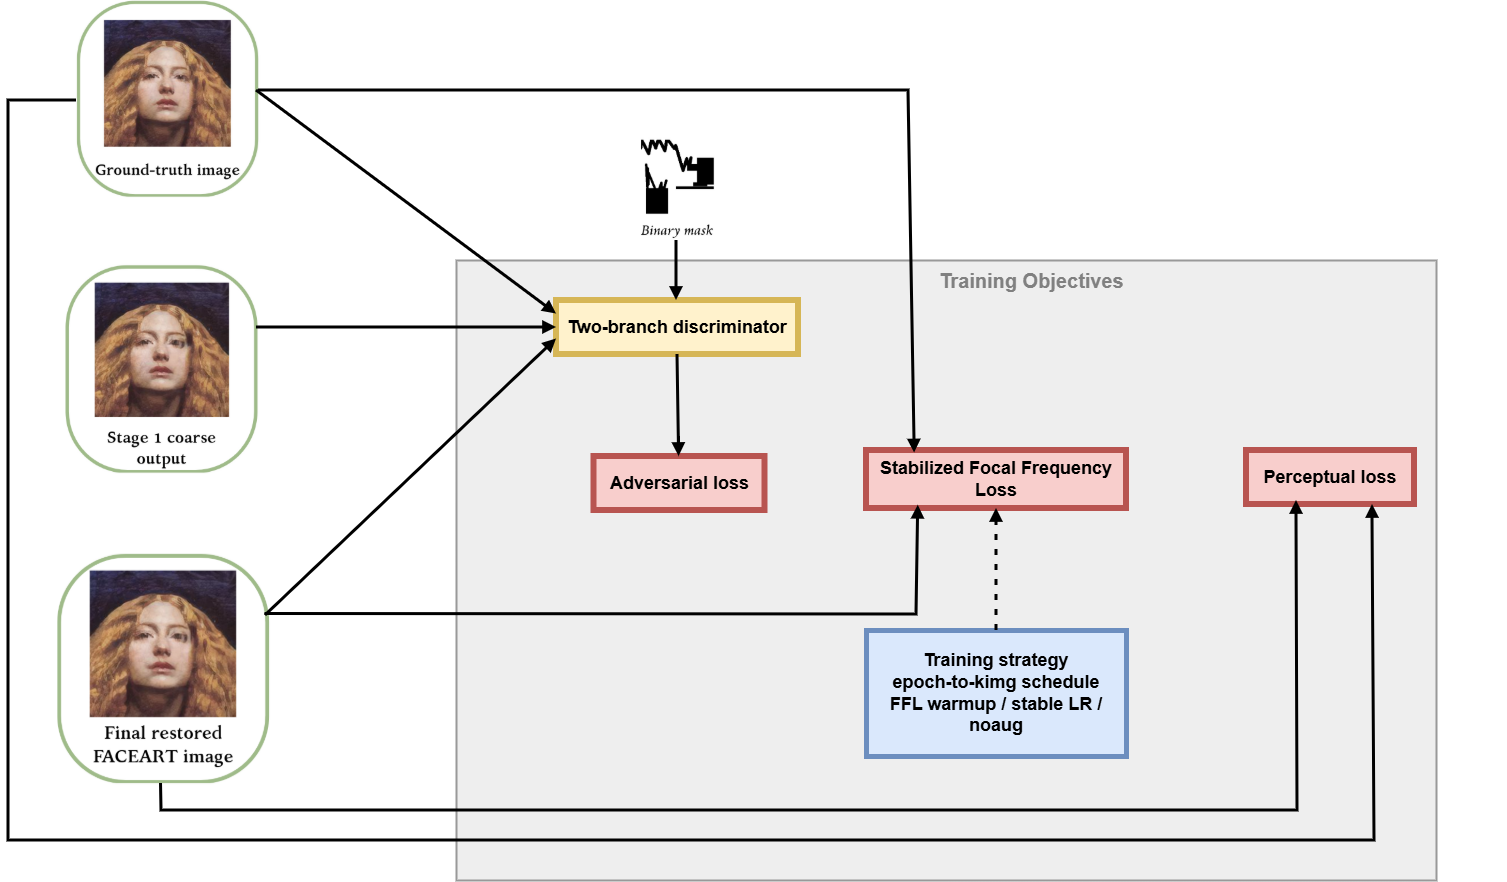
\includegraphics[width=1\linewidth]{fig3_9_training_objectives.png}%
    }{%
        \IfFileExists{fig3_9_training_objectives.png.png}{%
            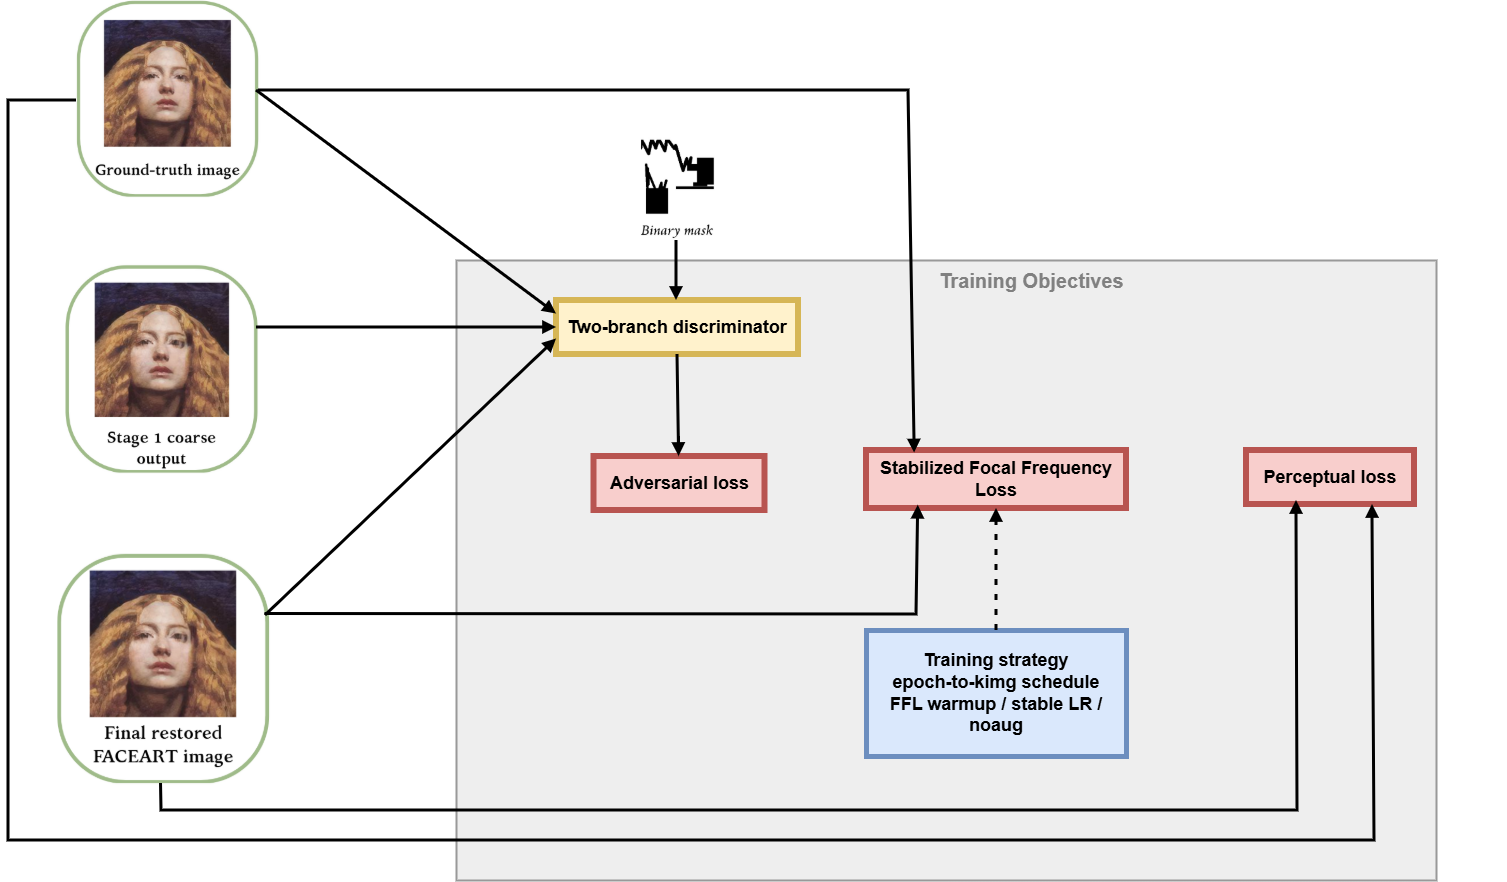
\includegraphics[width=1\linewidth]{fig3_9_training_objectives.png.png}%
        }{%
            \fbox{\parbox{0.92\linewidth}{\centering Placeholder for Figure 3.9\\Training objectives of PARF.}}%
        }%
    }
    \caption{Training objectives of PARF.}
    \label{fig:training_objectives}
\end{figure}

Figure~\ref{fig:training_objectives} summarizes the interaction between the main supervision terms used in the thesis methodology. The figure shows that PARF is optimized through a combination of adversarial loss, perceptual loss, and stabilized Focal Frequency Loss. Adversarial loss follows standard GAN-based realism supervision~\cite{goodfellow2014gan}, perceptual loss follows feature-space reconstruction supervision~\cite{johnson2016perceptual}, and the frequency-domain term is adapted from Focal Frequency Loss~\cite{jiang2021ffl}. The contribution of PARF is the way these losses are coordinated for a two-stage portrait-artwork restoration pipeline: adversarial and perceptual constraints maintain realism and semantic consistency, while the stabilized frequency-domain term emphasizes difficult high-frequency components that are important for painterly texture and facial detail. The figure is especially useful because it shows that the proposed optimization design is not centered on a single loss, but on the coordinated use of complementary constraints to guide both structural plausibility and fine-detail reconstruction.

% ------------------------------------------------------------
\subsection{Loss Functions}

The training process is formulated as a multi-objective optimization problem in which the restoration network is supervised by complementary losses. This thesis does not treat every loss term as a new invention. Instead, the loss design combines established supervision terms with a thesis-developed way of applying and coordinating them inside the PARF pipeline. Adversarial supervision and perceptual loss are retained from previous image synthesis and perceptual reconstruction literature~\cite{goodfellow2014gan,johnson2016perceptual}. The frequency-domain term follows the Focal Frequency Loss principle~\cite{jiang2021ffl}, but is adapted and stabilized for the portrait artwork setting.

The main contribution of PARF at the loss level is therefore the organization of these terms for a two-stage restoration framework. The losses are not applied as independent add-ons. They are used to supervise both coarse structural recovery and final refinement, so that the model is guided toward facial plausibility, painterly consistency, and frequency-sensitive texture restoration. This differs from a baseline loss setup that only optimizes a single final output with generic realism or feature-space constraints.

The overall objective of training is to produce restorations that are both semantically plausible and visually convincing, especially in portrait regions where structural mistakes are highly noticeable. In the proposed training formulation, the generator objective combines adversarial supervision on both stages with perceptual and frequency-domain constraints:
\begin{equation}
\mathcal{L}_{G}^{\mathrm{total}} =
\mathcal{L}_{G}^{(2)} + \mathcal{L}_{G}^{(1)} + \lambda_{p}\mathcal{L}_{P} + \lambda_{f}\mathcal{L}_{\mathrm{FFL}},
\end{equation}
where $\mathcal{L}_{G}^{(2)}$ and $\mathcal{L}_{G}^{(1)}$ denote adversarial losses for the final output and the Stage~1 output, respectively, $\mathcal{L}_{P}$ is the perceptual loss, and $\mathcal{L}_{\mathrm{FFL}}$ is the focal frequency loss.

% ------------------------------------------------------------
\noindent\textbf{Adversarial Supervision.}\par

Adversarial supervision is used to encourage the restoration network to produce realistic outputs that resemble real artwork images. The general adversarial formulation is inherited from GAN-based image synthesis~\cite{goodfellow2014gan}. PARF does not claim the adversarial loss itself as a new contribution. Its contribution is the way adversarial supervision is placed inside the proposed two-stage restoration design.

In a simpler baseline setting, adversarial loss may be applied only to the final generated image. In PARF, realism pressure is applied to both the final restored image and the Stage~1 coarse output through discriminator branches that evaluate restoration realism at different levels. This is important because the coarse output is not treated as a disposable intermediate result. It serves as the structural prior for Stage~2. Supervising it adversarially helps the framework avoid weak coarse layouts that would later limit refinement quality.

Following the non-saturating GAN formulation adopted in the proposed training design~\cite{goodfellow2014gan}, the generator-side adversarial losses are written as
\begin{equation}
\mathcal{L}_{G}^{(2)} = \mathbb{E}\big[\mathrm{softplus}(-D(\hat{\mathbf{I}}))\big],
\end{equation}
\begin{equation}
\mathcal{L}_{G}^{(1)} = \mathbb{E}\big[\mathrm{softplus}(-D^{(1)}(\hat{\mathbf{I}}^{(1)}))\big],
\end{equation}
where $D(\cdot)$ and $D^{(1)}(\cdot)$ denote the discriminator branches for the final restoration and the coarse Stage~1 output, respectively.

Similarly, the discriminator is trained with
\begin{equation}
\mathcal{L}_{D}^{\mathrm{fake}} =
\mathbb{E}\big[\mathrm{softplus}(D(\hat{\mathbf{I}}))\big] +
\mathbb{E}\big[\mathrm{softplus}(D^{(1)}(\hat{\mathbf{I}}^{(1)}))\big],
\end{equation}
\begin{equation}
\mathcal{L}_{D}^{\mathrm{real}} =
\mathbb{E}\big[\mathrm{softplus}(-D(\mathbf{I}))\big] +
\mathbb{E}\big[\mathrm{softplus}(-D^{(1)}(\mathbf{I}))\big].
\end{equation}
Following the R1 gradient-regularization strategy used to stabilize GAN training~\cite{mescheder2018training}, R1 regularization is applied to both discriminator branches:
\begin{equation}
\mathcal{L}_{R1}^{(2)} =
\frac{\gamma}{2}\, \mathbb{E}\left[\left\|\nabla_{\mathbf{I}} D(\mathbf{I})\right\|_2^2\right],
\end{equation}
\begin{equation}
\mathcal{L}_{R1}^{(1)} =
\frac{\gamma}{2}\, \mathbb{E}\left[\left\|\nabla_{\mathbf{I}} D^{(1)}(\mathbf{I})\right\|_2^2\right],
\end{equation}
\begin{equation}
\mathcal{L}_{R1}^{\mathrm{total}} = \mathcal{L}_{R1}^{(2)} + \mathcal{L}_{R1}^{(1)}.
\end{equation}

The practical role of this design is to discourage over-smoothed reconstructions and visually implausible completions. For portrait artwork restoration, this matters because a globally smooth face can still look artificial if the restored region lacks realistic tonal variation or facial detail. By supervising both restoration stages, PARF uses adversarial learning as part of a stage-wise training strategy rather than as a standalone borrowed loss.

% ------------------------------------------------------------
\noindent\textbf{Perceptual Loss.}\par

Perceptual loss is used to compare the restored output and the target artwork in a deep feature space rather than only at the pixel level. This idea follows perceptual reconstruction practice~\cite{johnson2016perceptual} and uses VGG-19 features as the feature extractor~\cite{simonyan2015vgg}. Therefore, the perceptual loss itself is an established component. PARF uses it as a necessary semantic and structural constraint within the proposed restoration objective.

The contribution in this thesis lies in how perceptual supervision is combined with the two-stage reconstruction process and the frequency-domain term. A baseline inpainting model may rely on perceptual loss mainly to improve general visual similarity. In PARF, perceptual loss is used to help preserve the semantic arrangement of portrait regions, especially the relationship among eyes, nose, mouth, facial contour, and surrounding painterly context. This is important because pixel-wise agreement alone may not capture whether a restored portrait remains visually credible.

Following prior perceptual reconstruction practice~\cite{johnson2016perceptual}, the perceptual loss is computed on VGG-19 features~\cite{simonyan2015vgg} as
\begin{equation}
\mathcal{L}_{P} = \sum_{i}\eta_i \left\|\phi_i(\hat{\mathbf{I}})-\phi_i(\mathbf{I})\right\|_1,
\end{equation}
where $\phi_i(\cdot)$ denotes the selected feature activations and $\eta_i$ are the layer weights. In this thesis, high-level VGG feature responses are used to emphasize semantic consistency and visually meaningful reconstruction quality, with the representative configuration focusing on \texttt{conv4\_4} and \texttt{conv5\_4} feature maps. This choice makes the loss more aligned with portrait-level structure than with low-level color matching alone.

% ------------------------------------------------------------
\vspace{0.35\baselineskip}
\noindent\textbf{Frequency-Domain Loss and Stability Design.}\par

Besides adversarial and perceptual losses, this thesis uses a frequency-domain supervision design built on the original Focal Frequency Loss (FFL) principle~\cite{jiang2021ffl}. The thesis does not claim the original FFL formulation as a new contribution. The contribution is the adaptation, integration, and stabilization of this frequency-domain idea for two-stage portrait artwork reconstruction.

The motivation is that artwork restoration is not only a semantic completion problem. Painted portraits contain soft shading, brush-like texture, tonal transitions, and fine facial details that can be weakened by spatial-domain supervision alone. Compared with a baseline loss setup that relies mainly on adversarial and perceptual constraints, the added frequency-domain term gives PARF an explicit mechanism for penalizing difficult spectral discrepancies. This helps the model pay more attention to high-frequency components that are visually important in restored facial regions.

Following the Focal Frequency Loss principle~\cite{jiang2021ffl}, the frequency-domain constraint used in PARF is written as
\begin{equation}
\mathcal{L}_{\mathrm{FFL}} = \mathcal{F}_{\mathrm{freq}}(\hat{\mathbf{I}}, \mathbf{I}),
\end{equation}
where $\mathcal{F}_{\mathrm{freq}}(\cdot,\cdot)$ denotes a frequency-domain discrepancy that emphasizes hard-to-reconstruct spectral components. In this thesis, the FFL term is coordinated with adversarial and perceptual supervision rather than used in isolation. This is the main difference from a direct off-the-shelf reuse of FFL. It allows PARF to preserve painterly texture while maintaining semantic facial structure and perceptual realism.

% ------------------------------------------------------------
\subsection{Optimization Strategy}

In addition to the loss design, PARF employs optimization strategies intended to improve convergence stability. These choices are not presented as new optimization algorithms. Adam optimization is adopted from established practice~\cite{kingma2015adam}, and R1 regularization follows prior work on stabilizing adversarial training~\cite{mescheder2018training}. The contribution of this thesis is the way these established tools are organized into a training recipe for the proposed two-stage portrait restoration framework.

The main difference from a simpler baseline training setup is the staged balance between structure-oriented and texture-oriented objectives. PARF first needs to learn stable coarse facial structure. It then needs to improve local facial detail and painterly texture without destabilizing the generated result. For this reason, the optimization strategy combines Adam-based training, schedule-controlled learning rates, R1 regularization, mask-aware bias, deterministic latent gating, and FFL warmup. Together, these choices support the proposed architecture and make the loss combination trainable as a whole.

In the proposed optimization strategy, the effective focal-frequency weight can be linearly warmed up as
\begin{equation}
\lambda_f^{\mathrm{eff}} =
\lambda_f \cdot \min\left(1,\frac{k_{\mathrm{img}}}{k_{\mathrm{warm}}}\right),
\end{equation}
where $k_{\mathrm{img}}$ is the current training progress measured in thousands of images and $k_{\mathrm{warm}}$ is the warmup length. This schedule allows the model to first stabilize coarse structural learning before placing stronger emphasis on frequency-domain refinement.

Additional stability choices in the proposed training design include mask-aware attention bias, deterministic latent gating at feature-latent blend points, and schedule-controlled learning-rate selection for short, medium, and long training regimes. This section focuses on the methodological rationale behind the optimization strategy rather than reporting convergence behavior or quantitative performance. Detailed experimental outcomes related to training will be presented later in Chapter~4.

\begin{table}[H]
\centering
\caption{Summary of training objectives and optimization settings.}
\label{tab:training_objectives_summary}
\begin{tabular}{p{0.28\linewidth} p{0.6\linewidth}}
\toprule
\textbf{Component} & \textbf{Description} \\
\midrule
Adversarial supervision & Non-saturating GAN loss applied to both the final Stage~2 output and the Stage~1 coarse output using a two-branch discriminator \\
Perceptual constraint & VGG-19 perceptual loss using \texttt{conv4\_4} and \texttt{conv5\_4} feature layers with weights $\tfrac{1}{4}$ and $\tfrac{1}{2}$ \\
Frequency-based constraint & Focal Frequency Loss for reducing spectral discrepancies and preserving painterly texture details \\
Optimization strategy & Adam optimizer with $\beta_1=0.0$, $\beta_2=0.99$, $\epsilon=10^{-8}$ and schedule-controlled learning rates for short, medium, and long training profiles \\
Stability mechanism & R1 regularization, mask-aware additive attention bias, deterministic latent gating, and optional FFL warmup over the first training kimg \\
\bottomrule
\end{tabular}
\end{table}

\begin{algorithm}[H]
\caption{PARF Inference and Training Procedure}
\label{alg:parf_procedure}
\begin{algorithmic}[1]
\Require Masked portrait artwork $I_m$, binary damage mask $M$, and visible known pixels $I_{\mathrm{known}}$
\Ensure Final restored portrait artwork $\hat{I}$
\State Concatenate $I_m$ and $M$ to form the restoration input.
\State Extract convolutional image--mask features from the input.
\State Estimate a coarse facial layout using the Stage~1 restoration path.
\State Apply mask-aware transformer reasoning and update token validity during Stage~1.
\State Generate the coarse restored estimate $\hat{I}_c$.
\State Preserve the visible known pixels and compose the Stage~2 input from $\hat{I}_c$, $I_{\mathrm{known}}$, and $M$.
\State Generate deterministic style guidance through the auxiliary noise--mapping--SMM path.
\State Inject the style guidance into the refinement bottleneck.
\State Refine the coarse result using the Stage~2 encoder--decoder.
\State Produce the final restored portrait artwork $\hat{I}$.
\If{training mode}
    \State Compute reconstruction and perceptual supervision for $\hat{I}_c$ and $\hat{I}$.
    \State Apply adversarial supervision to improve visual realism.
    \State Apply stabilized Focal Frequency Loss to encourage frequency-sensitive texture recovery.
    \State Update PARF parameters by minimizing the combined training objective.
\EndIf
\State \Return $\hat{I}$
\end{algorithmic}
\end{algorithm}

Algorithm~\ref{alg:parf_procedure} converts the PARF workflow for portrait artwork reconstruction into pseudocode. Unlike Figure~\ref{fig:framework_overview}, which shows the complete architecture visually, the algorithm states the ordered computation performed by the method. The procedure begins with a masked FACEART portrait and its binary mask. The visible known pixels are kept as contextual evidence, while the masked image and mask are encoded into convolutional image--mask features.

The first part of the algorithm corresponds to Stage~1. This stage estimates the coarse facial layout and updates token validity during mask-aware transformer reasoning. Its goal is not to produce the final high-quality restoration immediately, but to recover a structurally plausible facial arrangement that can guide the later refinement stage.

The second part corresponds to Stage~2. The coarse result is combined with the visible known pixels and the mask, then refined by an encoder--decoder path. The auxiliary noise--mapping--SMM branch produces deterministic style guidance and injects it at the refinement bottleneck. This branch does not replace the main restoration path. It acts as a modulation signal that helps the refined output remain consistent with the painterly appearance of the input portrait.

The final conditional block separates training from inference. During training, PARF uses reconstruction, perceptual, adversarial, and stabilized Focal Frequency Loss supervision to learn structural plausibility and frequency-sensitive texture recovery. During inference, the loss computation is removed. The model only follows the forward procedure from input preparation to final restored portrait generation.

% ------------------------------------------------------------
\section{Chapter Summary}

This chapter presented the methodological design of PARF, the proposed Portrait Artwork Reconstruction Framework for face-centered artwork inpainting. The chapter first clarified the overall restoration pipeline and explained how a damaged portrait artwork is represented by the masked input image and the corresponding binary mask. This input formulation is important because the framework must distinguish between reliable visible pixels and missing regions that require reconstruction. From this starting point, the chapter described PARF as a coarse-to-refinement system rather than a single-step restoration model.

The first major part of the methodology focused on Stage~1, where the framework estimates a coarse but structurally meaningful restoration result. This stage is responsible for recovering the global facial layout, preserving the visible context, and producing an initial reconstruction that can guide the later refinement process. The chapter also explained the role of transformer-based reasoning, mask-guided validity propagation, and mask updating in supporting large-hole reconstruction. These mechanisms allow the model to reason across visible and missing regions while maintaining awareness of which tokens are derived from reliable image content and which tokens correspond to uncertain restored areas.

The second major part of the chapter described the thesis-specific refinement direction of PARF. Instead of relying only on the coarse output, the framework introduces a Stage~2 refinement path that uses the Stage~1 result, known visible pixels, and mask information as a more informative input state. This refinement stage is designed to improve local facial plausibility and painterly consistency after the global layout has already been estimated. The chapter further discussed the auxiliary style guidance pathway, deterministic latent modulation, and bottleneck-level fusion strategy, which together help the refinement decoder preserve the visual character of portrait artwork while improving the reconstructed facial region.

Finally, the chapter explained the training objective and optimization design used to support the proposed restoration framework. The combination of reconstruction, perceptual, adversarial, and stabilized Focal Frequency Loss components reflects the need to optimize both low-level fidelity and visually meaningful details. This is especially relevant for portrait artwork reconstruction because the restored result must appear coherent not only at the pixel level but also in terms of facial structure, brush-like texture, and perceptual realism. Overall, Chapter~3 established the technical foundation for PARF and clarified how its main contribution lies in organizing inherited inpainting mechanisms and thesis-developed refinements into a portrait-artwork-oriented restoration framework. Based on this methodology, Chapter~4 evaluates whether the proposed design produces measurable and visually meaningful improvements in practice.

\chapter{Experiments and Results}

\section{Implementation Details}

This chapter presents the practical implementation of PARF and the experimental evaluation used to assess it on portrait artwork restoration. Chapter~3 focused on methodological design. By contrast, this chapter concentrates on implementation settings, dataset preparation, restoration results, baseline comparison, and evaluation of the resulting outputs.

\vspace{0.35\baselineskip}
\noindent\textbf{Development Environment.}\par

The implementation environment is summarized first because reproducibility depends strongly on the software stack and hardware configuration used to train and evaluate the model. PARF was implemented in Python with PyTorch and executed on a CUDA-enabled GPU environment. Table~\ref{tab:dev_environment} reports the main programming language, deep learning framework, CUDA and cuDNN versions, GPU model, operating environment, and supporting libraries used during experimentation.

\begin{table}[H]
\centering
\caption{Development environment used for implementation and experimentation.}
\label{tab:dev_environment}
\begin{tabular}{>{\raggedright\arraybackslash}p{0.32\linewidth} >{\raggedright\arraybackslash}p{0.56\linewidth}}
\toprule
\textbf{Component} & \textbf{Description} \\
\midrule
Programming language & Python 3.8.20 \\
Deep learning framework & PyTorch 1.9.1+cu111 \\
CUDA / cuDNN & CUDA 11.1 and cuDNN 8.0.5 \\
GPU / hardware & NVIDIA A100-SXM4-80GB \\
Operating environment & Ubuntu 24.04.4 LTS (Linux) \\
Supporting libraries & torchvision 0.10.1+cu111, NumPy 1.24.4, OpenCV 4.13.0.92, SciPy 1.10.1, scikit-image 0.21.0, timm 0.4.12, and matplotlib 3.7.5 \\
\bottomrule
\end{tabular}
\end{table}

\vspace{0.35\baselineskip}
\noindent\textbf{Model and Training Configuration.}\par

The practical training configuration is then reported to clarify how the methodology described in Chapter~3 was executed in the experimental workflow. The configuration includes the unified input resolution, optimizer settings, learning-rate behavior, batch size, training duration, checkpoint strategy, and the major objective weights used in the representative thesis run. These details are listed in Table~\ref{tab:train_config} to document the experimental setup without repeating the methodological rationale already discussed in the previous chapter.

\begin{table}[H]
\centering
\caption{Model and training configuration used in the experiments.}
\label{tab:train_config}
\begin{tabular}{>{\raggedright\arraybackslash}p{0.32\linewidth} >{\raggedright\arraybackslash}p{0.56\linewidth}}
\toprule
\textbf{Setting} & \textbf{Description} \\
\midrule
Image resolution & 512 $\times$ 512 input images using the \texttt{dataset\_512} pipeline with the \texttt{places512} configuration \\
Optimizer & Adam for both generator and discriminator; representative learning rates are $5\times10^{-5}$ for the main optimization path and $1\times10^{-4}$ for the transformer subgroup \\
Learning-rate schedule & Fixed learning rates during training in the representative thesis run; although the repository supports profile-based defaults, the thesis run explicitly overrides them with fixed \texttt{lr} and \texttt{lrt} settings \\
Batch size & 4 \\
Training duration & 40 epochs, corresponding to approximately 151 kimg in the representative thesis training configuration \\
Checkpoint setting & Training is initialized from a previously saved \texttt{network-snapshot-*.pkl} checkpoint and then continued for further optimization, with periodic snapshots saved every 2 ticks \\
Major objective weights & Two-stage adversarial objective with perceptual ratio $0.1$ and focal-frequency ratio $0.02$; path-length regularization is disabled, and the representative \texttt{places512} configuration uses R1 $\gamma = 10$ \\
\bottomrule
\end{tabular}
\end{table}

\vspace{0.35\baselineskip}
\noindent\textbf{Inference Configuration.}\par

During inference, each test image is paired with a prepared binary mask, passed through the trained restoration model, and exported for qualitative inspection and comparative analysis. The inference outputs are organized so that the same samples can later be reused for selected-result presentation, direct baseline comparison, and visual checkpoint-based ablation analysis.

To keep the comparison fair and reproducible, the inference stage preserves stable filename mapping between the original image, the masked input, and the restored output. This organization is especially important for the thesis workflow because the same test cases are referenced repeatedly in the selected-result gallery, the side-by-side comparison figures, and the failure-case analysis.

\section{Dataset Preparation}

\vspace{0.35\baselineskip}
\noindent\textbf{Artwork Dataset Preparation.}\par

This section describes the portrait-artwork data prepared for Chapter~4 experiments. The evaluation images are drawn from the thesis artwork collection and are organized so that the same samples can be reused consistently for result presentation, comparison, and later evaluation. In line with the portrait-oriented scope of this thesis, the selected samples emphasize visible faces, upper-body portrait compositions, and painterly styles in which local facial errors are easy to perceive.

The use of artwork images rather than natural photographs remains important at the experimental stage because the restoration task must preserve both semantic plausibility and artistic continuity. Consequently, the data preparation process keeps a unified resolution setting and stable filename mapping so that each original image can be paired consistently with masked inputs, proposed outputs, and baseline outputs throughout the comparison workflow. In the representative thesis setup, the training and validation corpus follows the same portrait-artwork collection used in Chapter~3, while a smaller curated evaluation subset is prepared separately for the visual results and comparative figures in this chapter.

\begin{figure}[H]
    \centering
    \includegraphics[width=0.92\linewidth]{fig4_1_eval_samples.png}
    \caption{Representative artwork samples prepared for experimental evaluation.}
    \label{fig:eval_samples}
\end{figure}

Figure~\ref{fig:eval_samples} shows representative portrait artwork samples selected for experimental evaluation. These examples are included to demonstrate the visual domain targeted by the thesis: painted or painterly portraits in which facial structure, skin-tone transition, hair texture, and background style must remain coherent after restoration. The figure also clarifies that the evaluation is not focused on generic natural images, but on artwork cases where small facial distortions are visually noticeable. This makes the selected samples suitable for testing whether PARF can preserve both portrait structure and artistic appearance.

\begin{table}[H]
\centering
\caption{Summary of the artwork data prepared for Chapter~4 experiments.}
\label{tab:eval_dataset_summary}
\begin{tabular}{p{0.28\linewidth} p{0.6\linewidth}}
\toprule
\textbf{Property} & \textbf{Description} \\
\midrule
Image domain & Portrait artworks / face-oriented paintings \\
Image type & Digitized RGB artwork images organized for training, validation, and curated evaluation reuse \\
Target task & Portrait artwork restoration under masked damage \\
Resolution & $512 \times 512$ unified preparation setting \\
Representative split & 3758 training images, 304 validation images, with a separate curated evaluation subset prepared for qualitative results, comparison, and later analysis \\
\bottomrule
\end{tabular}
\end{table}

\vspace{0.35\baselineskip}
\noindent\textbf{Damage-Mask Preparation.}\par

This section describes the damage masks prepared for Chapter~4 experiments. The evaluation protocol follows the same portrait-artwork restoration setting established in Chapter~3, but the practical preparation here emphasizes stable reuse of fixed masks for fair comparison across all methods. In this way, every model is tested on the same masked regions rather than on separately randomized masks.

The prepared masks retain the large-hole and irregular-boundary characteristics required for challenging artwork reconstruction while also allowing controlled visual comparison on face-sensitive regions. This preparation makes it possible to discuss both qualitative behavior and comparative performance under identical missing-region conditions. In addition to the stochastic masks used during training, the evaluation workflow fixes the selected mask assets in advance so that PARF, MAT baseline, and other comparison methods receive exactly the same masked inputs.

\begin{figure}[H]
    \centering
    \includegraphics[width=0.92\linewidth]{fig4_2_eval_masks.png}
    \caption{Prepared damage masks and masked artwork inputs used in the experiments.}
    \label{fig:eval_masks}
\end{figure}

Figure~\ref{fig:eval_masks} presents the prepared masks and masked artwork inputs used during evaluation. The masks are intentionally placed over visually important portrait regions so that the restoration task tests more than simple background filling. By showing both the binary mask and the resulting masked input, the figure makes clear which image regions are removed and what visual context remains available to the model. This is important for fair comparison because all evaluated methods receive the same masked inputs, allowing differences in the final outputs to be attributed to the restoration behavior of each method rather than to different damage patterns.

\begin{table}[H]
\centering
\caption{Summary of the damage-mask preparation used in Chapter~4 experiments.}
\label{tab:eval_mask_summary}
\begin{tabular}{p{0.28\linewidth} p{0.6\linewidth}}
\toprule
\textbf{Setting} & \textbf{Description} \\
\midrule
Mask type & Free-form irregular binary masks, together with fixed evaluation masks prepared for direct cross-method comparison \\
Coverage design & Large-hole and center-focused missing regions selected to remain challenging without trivializing the portrait reconstruction task \\
Target region & Corruption patterns designed to overlap frequently with semantically important facial areas \\
Experimental use & Shared masked inputs reused across selected-result presentation, comparison figures, and later evaluation \\
\bottomrule
\end{tabular}
\end{table}

\section{Results and Discussion}

\vspace{0.35\baselineskip}
\noindent\textbf{Selected Restoration Results.}\par

This section presents the restoration outputs produced by PARF itself before placing them in direct comparison with other methods. The result figure is consolidated from the previous selected-result and stage-wise visualizations so that the reader can observe both the restoration output and the internal two-stage behavior in one place. This avoids repeating two highly related figures while still preserving the essential qualitative evidence: the original reference, the masked input, the Stage~1 coarse output, and the final restored result after Stage~2 refinement.

The selected cases do not replace the later comparison and evaluation sections. Their role is simpler. They show how PARF behaves on representative portrait-artwork samples before the discussion moves to external baselines. The figure therefore serves as the main qualitative presentation in this section. The discussion focuses on facial plausibility, painterly continuity, boundary integration, and the transition from coarse reconstruction to refined restoration.

\begin{figure}[p]
    \centering
    \includegraphics[width=0.95\linewidth,height=0.78\textheight,keepaspectratio]{fig4_4_stagewise_results.png}
    \caption{Qualitative restoration results of PARF.}
    \label{fig:proposed_results}
\end{figure}
\clearpage

Figure~\ref{fig:proposed_results} presents the main qualitative results of PARF and includes the intermediate Stage~1 output. This makes the restoration process easier to interpret. Each row contains the original portrait, the masked input, the Stage~1 output, and the final restored result. The original image provides the reference appearance. The masked input shows the damaged facial region. The Stage~1 output is the coarse prediction. At this point, the framework estimates the main facial structure and produces a globally plausible completion. This intermediate result is not the final goal. Its purpose is to recover the broad spatial arrangement of the missing region and provide a stable base for later refinement.

The final result shows the effect of the refinement stage. Compared with the Stage~1 output, it improves local tone transitions, reduces boundary discontinuities, and produces a more coherent painterly appearance. In several examples, Stage~1 already recovers the approximate facial layout. The final result then looks smoother and better integrated with the surrounding artwork. This distinction matters because PARF does not rely on a single-pass reconstruction strategy. The final quality depends on cooperation between global reasoning in Stage~1 and local refinement in Stage~2. This behavior is important for portrait artwork restoration, where the model must reconstruct sensitive facial components while keeping the repaired area compatible with the surrounding style.

\vspace{0.35\baselineskip}
\noindent\textbf{Discussion of Representative Results.}\par

The representative cases in Figure~\ref{fig:proposed_results} are discussed here with emphasis on facial alignment, restoration of semantically important regions, and painterly consistency. Strong cases usually reflect effective coarse completion followed by successful refinement. Weaker cases appear more often when the missing region is highly ambiguous or when the painterly texture is difficult to reconstruct.

In practical terms, the strongest results are those in which the reconstructed face remains coherent at both the global and local levels. The facial contour stays plausible. The main facial parts remain correctly arranged. The restored region also blends with the surrounding painterly style. These examples suggest that the two-stage design works best when the missing area disrupts the central face but still leaves enough visible context for Stage~1 reasoning and Stage~2 refinement to cooperate. Under those conditions, the outputs tend to preserve facial plausibility, tone transition, brushstroke continuity, and boundary smoothness.

These results should still be read as strong cases rather than a complete characterization of the model under every damage scenario. Some samples show mild oversmoothing or reduced sharpness in ambiguous areas. This occurs more often when the painterly texture is irregular or when the missing region removes too much structural evidence. The discussion therefore serves as a bridge between the PARF-only results in this section and the cross-method comparison in Section~4.4.

\section{Comparison}

\subsection{Baseline Methods}

This section identifies the methods selected for comparative analysis and clarifies why they are relevant to portrait artwork reconstruction. The original MAT model remains the primary baseline because it is the architectural foundation on which the thesis-developed framework is built. To make the comparison academically stronger, the analysis additionally includes ZITS as a structure-guided transformer model~\cite{zeng2022zits}, RePaint as a diffusion-based inpainting method~\cite{lugmayr2022repaint}, LaMa as a Fourier-convolution restoration model~\cite{suvorov2022lama}, and RAD as a recent region-aware diffusion method~\cite{kim2025rad}. Together, these methods represent several distinct paradigms for damaged-image completion: semantic transformer reasoning, explicit structure modeling, stochastic diffusion sampling, region-aware diffusion scheduling, and large-receptive-field Fourier convolution.

\begin{table}[H]
\centering
\caption{Baseline methods used for comparison in the experiments.}
\label{tab:baselines}
\begin{tabular}{p{0.28\linewidth} p{0.6\linewidth}}
\toprule
\textbf{Method} & \textbf{Description} \\
\midrule
ZITS~\cite{zeng2022zits} & Structure-guided transformer inpainting that predicts contour-related structure cues before texture completion, making it a strong reference for face and contour reconstruction \\
RePaint~\cite{lugmayr2022repaint} & Diffusion-based inpainting that keeps valid pixels fixed while iteratively resampling the masked region, offering strong perceptual realism and global coherence \\
LaMa~\cite{suvorov2022lama} & Fourier-convolution inpainting model with large receptive fields and efficient fully convolutional inference, serving as a strong large-hole restoration baseline \\
RAD~\cite{kim2025rad} & Region-Aware Diffusion model that improves diffusion inpainting efficiency through region-aware noise scheduling and a simplified reverse process, although it does not explicitly model portrait-specific structure or artistic coherence \\
MAT baseline~\cite{li2022mat} & Original Mask-Aware Transformer for large-hole image inpainting, combining convolutional feature extraction, mask-aware transformer reasoning, dynamic mask updating, and style-modulated reconstruction \\
PARF & Thesis-developed portrait artwork reconstruction framework built on a transformer-based inpainting foundation, extended with deep-stage residual adapters, deterministic latent guidance, dedicated Stage~2 refinement, and frequency-domain training design \\
\bottomrule
\end{tabular}
\end{table}

For fair comparison, all methods were evaluated on the same portrait-artwork samples, under the same damage-mask settings, and with the same quantitative metrics. Official papers, official repositories, and publicly released pretrained checkpoints were used whenever available so that the comparison reflects the original design intent of each method rather than unofficial reimplementations.

\subsection{Quantitative Comparison}

This section presents the quantitative performance of PARF against the original MAT baseline~\cite{li2022mat} and the selected recent methods, namely ZITS~\cite{zeng2022zits}, RePaint~\cite{lugmayr2022repaint}, LaMa~\cite{suvorov2022lama}, and RAD~\cite{kim2025rad}. The main table summarizes restoration quality under the chosen metrics. MAT is kept as the main architectural reference, while the newer methods serve as contemporary comparison points.

The purpose of the quantitative comparison is not only to test whether PARF improves over the original MAT baseline. It is also to show how the framework behaves relative to methods built on different restoration paradigms. This allows the thesis to discuss the results from the viewpoints of pixel fidelity, structural consistency, and perceptual realism together.

\begin{table}[H]
\centering
\caption{Quantitative comparison of restoration performance against baselines and recent methods.}
\label{tab:quant_results}
\begin{tabular}{p{0.24\linewidth} c c c}
\toprule
\textbf{Method} & \textbf{PSNR} & \textbf{SSIM} & \textbf{LPIPS} \\
\midrule
ZITS & 35.3964 & 0.9783 & 0.0243 \\
RePaint & 29.4532 & 0.9560 & 0.0597 \\
LaMa & 35.2210 & \textbf{0.9784} & 0.0231 \\
RAD & 24.5721 & 0.9175 & 0.1400 \\
MAT baseline & 34.8529 & 0.9766 & 0.0228 \\
PARF (proposed) & \textbf{35.4292} & 0.9776 & \textbf{0.0183} \\
\bottomrule
\end{tabular}
\end{table}

Table~\ref{tab:quant_results} reports the average quantitative performance of each method across the evaluated samples. PARF achieves the highest PSNR and the lowest LPIPS among the compared methods. Under the present evaluation protocol, this suggests stronger reconstruction fidelity and better perceptual similarity. In direct comparison with the original MAT baseline, PARF raises PSNR from 34.8529 to 35.4292. It also increases SSIM from 0.9766 to 0.9776 and reduces LPIPS from 0.0228 to 0.0183. Taken together, these results support the view that the thesis-developed extensions improve both reconstruction accuracy and visual quality.

Among the recent comparison methods, ZITS and LaMa remain highly competitive in structural similarity. LaMa achieves the highest SSIM by a narrow margin. RAD performs below the strongest transformer and Fourier-convolution baselines in this portrait-artwork evaluation. This result is consistent with its design goal. RAD is primarily an efficient region-aware diffusion method, not a model tailored to portrait structure or artistic detail. It improves diffusion inpainting through region-aware noise scheduling and a simplified reverse process. However, it does not explicitly introduce portrait-specific structure priors or artwork-oriented refinement.

Overall, PARF provides the most balanced profile across the three reported metrics. It leads in pixel-level fidelity and perceptual quality while remaining close to the strongest SSIM result. This pattern is meaningful for portrait artwork restoration, where a convincing output must preserve structure, painterly appearance, and fine facial detail at the same time.

\subsection{Qualitative Comparison}

This section compares the visual behavior of PARF against the original MAT baseline~\cite{li2022mat} and the selected recent methods ZITS~\cite{zeng2022zits}, RePaint~\cite{lugmayr2022repaint}, LaMa~\cite{suvorov2022lama}, and RAD~\cite{kim2025rad} on representative portrait artwork samples. Section~4.3 only presented PARF outputs. Here, the same evaluation cases are placed side by side so that differences in structure, detail, and style preservation can be assessed directly.

The qualitative comparison is especially important for portrait artwork reconstruction because metric improvements alone do not always capture whether a result looks visually convincing. Side-by-side inspection helps reveal whether PARF preserves facial plausibility and artistic continuity more reliably than the comparison methods.

\begin{figure}[H]
    \centering
    \includegraphics[width=0.98\linewidth,height=0.87\textheight,keepaspectratio]{fig4_5_qual_compare.png}
    \caption{Qualitative comparison of PARF, MAT, and recent baselines.}
    \label{fig:qual_compare}
\end{figure}
\clearpage

Figure~\ref{fig:qual_compare} compares the visual behavior of each method under identical masked inputs. The rows show how different paradigms respond to the same portrait-artwork damage. Some methods produce overly smooth completions. Some introduce structural distortion. Others preserve texture but fail to align facial details convincingly. MAT baseline remains an important reference because it supplies the transformer foundation. ZITS, RePaint, LaMa, and RAD represent structure-guided, diffusion, Fourier-convolution, and region-aware diffusion alternatives.

In the updated comparison, RAD produces visible color artifacts and noisy local content in several masked facial regions. This suggests that its default restoration process is not sufficiently constrained for portrait artwork structure or painterly facial coherence. Across the representative samples, PARF preserves facial coherence more reliably than the weaker comparison cases. It also remains visually competitive with the strongest alternatives. In most examples, it gives a more balanced combination of restored detail, contour stability, and painterly continuity around the masked region.

\section{Evaluation}

\subsection{Evaluation Metrics}

This section defines the quantitative and perceptual metrics used for experimental assessment. In the present thesis, the evaluation focuses on PSNR, SSIM, and LPIPS so that pixel accuracy, structural consistency, and perceptual similarity can be discussed together rather than through a single criterion alone.

This combination of metrics is used because no single evaluation criterion is sufficient for portrait artwork restoration. A model may achieve strong pixel-level accuracy without producing the most convincing perceptual appearance, and conversely, a visually pleasing result may not always maximize pixel similarity. Using PSNR, SSIM, and LPIPS together therefore provides a more balanced interpretation of restoration quality.

\begin{table}[H]
\centering
\caption{Evaluation metrics used to assess restoration performance.}
\label{tab:metrics}
\begin{tabular}{p{0.28\linewidth} p{0.6\linewidth}}
\toprule
\textbf{Metric} & \textbf{Purpose} \\
\midrule
PSNR & Measures pixel-level reconstruction fidelity by comparing the restored image with the reference image in terms of signal-to-noise ratio; higher values indicate more accurate pixel recovery \\
SSIM & Measures structural similarity between the restored image and the reference image, with emphasis on luminance, contrast, and local structural consistency; higher values indicate better structural preservation \\
LPIPS & Measures perceptual similarity using deep visual features rather than raw pixels, making it useful for judging whether the restored result looks visually close to the reference image; lower values indicate better perceptual quality \\
\bottomrule
\end{tabular}
\end{table}

In the present thesis protocol, these three metrics are computed on the full restored image rather than only on the masked region, using the paired ground-truth artwork as reference. The reported values are averaged over the prepared thesis evaluation set under the same evaluation setting, while filename remapping is applied where necessary so that outputs from every model are paired with the correct reference image. LPIPS is evaluated with AlexNet-based features after standard normalization to the $[-1,1]$ range.

\subsection{Ablation Study}

This section uses the available thesis checkpoints as practical ablation evidence for PARF. These checkpoints do not isolate every component through fully independent removal runs. Even so, they still show how restoration quality changes as the design gradually adds frequency-aware training and later architectural extensions.

In this interpretation, the Focal Frequency Loss (FFL) checkpoint represents the earliest frequency-aware training stage, before the later thesis-specific architectural additions are introduced. The Phase~1 architecture reflects the first architecture-level extension. The Phase~2 architecture represents a more advanced refinement-oriented version of the design. Taken together, these checkpoints show how restoration quality evolves as the framework accumulates both training-level and architecture-level improvements.

\begin{table}[H]
\centering
\caption{Checkpoint-based ablation comparison of the selected thesis checkpoints under the prepared evaluation setting.}
\label{tab:phasewise_quant}
\begin{tabular}{p{0.38\linewidth} c c c}
\toprule
\textbf{Configuration} & \textbf{PSNR} & \textbf{SSIM} & \textbf{LPIPS} \\
\midrule
FFL checkpoint & 33.1737 & 0.9719 & 0.0323 \\
Phase~1 architecture & 35.2588 & 0.9781 & 0.0189 \\
Phase~2 architecture & \textbf{35.4513} & \textbf{0.9782} & \textbf{0.0186} \\
\bottomrule
\end{tabular}
\end{table}

Table~\ref{tab:phasewise_quant} shows a clear improvement trend across the selected thesis checkpoints under the prepared evaluation setting. The Focal Frequency Loss (FFL) checkpoint provides the earliest frequency-aware training baseline, but both later architecture stages improve substantially over it in all three metrics. In particular, the transition from the FFL checkpoint to Phase~1 produces a strong gain in PSNR and SSIM together with a large reduction in LPIPS, indicating that the first thesis-specific architectural extension contributes meaningfully to both reconstruction fidelity and perceptual quality.

The Phase~2 architecture then achieves the best result among the three checkpoints, with further gains in PSNR and SSIM and the lowest LPIPS value. Although the improvement from Phase~1 to Phase~2 is smaller than the earlier jump from the FFL checkpoint to Phase~1, the result remains consistent across all reported metrics. This pattern supports the interpretation that PARF benefits not only from the proposed frequency-aware training design, but also from the later refinement-oriented architectural development introduced in the final internal phases.

\begin{figure}[H]
    \centering
    \includegraphics[width=0.98\linewidth,height=0.80\textheight,keepaspectratio]{fig4_6_phasewise_visual.png}
    \caption{Visual checkpoint-based ablation comparison of the selected thesis checkpoints.}
    \label{fig:phasewise_visual}
\end{figure}

Figure~\ref{fig:phasewise_visual} provides visual support for the same progression observed in Table~\ref{tab:phasewise_quant}. The figure should be interpreted as a checkpoint-based ablation visualization: each row corresponds to a different internal development stage, and the comparison focuses on how restoration quality changes as the framework becomes more complete. The FFL checkpoint already produces globally plausible restorations, but its outputs remain comparatively softer and less stable around the reconstructed facial region. The Phase~1 architecture improves this behavior by producing clearer facial structure, more reliable contour recovery, and better integration between the restored area and the surrounding painterly context. The Phase~2 architecture then offers the most refined visual result among the three checkpoints, with improved local coherence and a more convincing balance between facial plausibility and artistic continuity. This visual trend is consistent with the reported metrics and strengthens the interpretation that PARF benefits from both the earlier frequency-aware training stage and the later architecture-level refinements.

\subsection{Limitation}

This section describes the cases in which PARF remains limited, such as severe structural ambiguity, extreme damage, oversmoothing, or style inconsistency under difficult restoration scenarios. The goal is to connect the observed weaknesses directly to the empirical evidence instead of leaving them only to the final conclusion chapter.

These limitations are still valuable from an evaluation perspective because they mark the boundary of the current thesis design. By identifying the kinds of damaged portrait artworks that remain difficult, the chapter can distinguish between the strengths of PARF and the cases that still require future improvement.

\begin{figure}[H]
    \centering
    \includegraphics[width=0.98\linewidth,height=0.80\textheight,keepaspectratio]{fig4_7_failure_cases.png}
    \caption{Failure cases and remaining limitations of PARF.}
    \label{fig:failure_cases}
\end{figure}

Figure~\ref{fig:failure_cases} presents representative failure cases of PARF under particularly difficult portrait-artwork restoration conditions. In these examples, the masked region covers either nearly the entire facial area or more than half of the semantically important facial components, such as the eyes, upper nose region, and central facial contour. Under this degree of corruption, the restoration task becomes much more ambiguous because the network must infer a large proportion of identity-defining and structure-critical content from only limited surrounding evidence.

Even in these difficult cases, PARF still preserves several coarse portrait-level properties. The restored outputs remain broadly consistent with the original head shape, approximate facial placement, hair silhouette, and overall color distribution of the artwork. This behavior suggests that the framework still retains useful global reasoning capacity and can generate a face-like completion rather than collapsing into unrelated visual artifacts. From an evaluation perspective, this partial robustness remains important because it shows that the model does not fail completely when the damaged region becomes unusually large.

At the same time, the visual results also reveal a clear limitation of the current thesis design. When the mask removes most of the key facial components, the model no longer has enough reliable evidence to recover fine anatomical relationships with high confidence. As a result, local errors become more noticeable in the reconstructed eyes, nose bridge, and surrounding facial boundaries. In the first case, the restored eye region and upper-face structure are no longer fully aligned with the original portrait, and the reconstructed facial details appear distorted and incomplete. In the second case, the output remains smoother and more coherent at the global level, but the recovered facial components still lack the precision and sharpness required for a convincing high-fidelity restoration. These examples indicate that PARF is better at preserving coarse facial plausibility than at reconstructing exact fine-grained identity cues when the masked region becomes too dominant.

This limitation is consistent with the broader design assumptions of PARF. The model performs best when at least a meaningful portion of the surrounding facial structure remains visible, allowing Stage~1 to infer a stable global layout and Stage~2 to refine local details from that coarse estimate. When this structural support is heavily reduced, the restoration problem gradually shifts from guided completion toward highly uncertain generation, and the final output becomes less reliable. Therefore, the cases in Figure~\ref{fig:failure_cases} should not be interpreted as contradictions of the overall effectiveness of PARF. Instead, they define the practical boundary conditions under which PARF begins to lose fine-detail accuracy. This observation is important not only for a balanced interpretation of the thesis contribution, but also for motivating future improvements based on stronger face-structure priors, more explicit semantic guidance, or training strategies designed specifically for severe face-dominant occlusion.

\section{Chapter Summary}

This chapter presented the practical implementation and experimental evaluation of PARF for portrait artwork reconstruction. It first described the implementation environment, training configuration, and inference setting used throughout the experiments. These details matter because the reported results depend not only on the model architecture, but also on resolution, checkpoint selection, input preparation, and evaluation protocol. By documenting these conditions, the chapter establishes a clear basis for interpreting the qualitative and quantitative findings.

The chapter then explained the dataset preparation process and the construction of damaged portrait inputs. The evaluation focuses on portrait artworks rather than generic natural images because the thesis is concerned with semantically important facial regions. The discussion of artwork preparation and mask generation shows why the setting is challenging. The missing regions often affect the eyes, nose, mouth, facial contour, and nearby painterly transitions. These areas require the model to reconstruct both structure and appearance, which makes the task more demanding than simple texture filling.

After establishing the experimental setting, the chapter presented qualitative restoration results of PARF. The selected examples show that the framework can preserve the broad portrait composition while reconstructing missing facial regions in a visually coherent way. The stage-wise results also support the methodology introduced in Chapter~3. They show how the coarse output provides an initial facial layout and how the refinement stage improves local detail and visual continuity. These findings matter because portrait artwork restoration cannot be judged by numerical scores alone. Anatomical plausibility, painterly consistency, and natural integration with visible context are also essential.

The quantitative comparison further demonstrated the effectiveness of PARF under the selected thesis protocol. PARF achieved the strongest overall metric profile when compared with the selected transformer, diffusion, Fourier-convolution, and region-aware diffusion baselines. The metrics suggest that the framework provides a favorable balance between pixel-level fidelity, structural similarity, and perceptual quality. The checkpoint-based ablation study also showed a consistent improvement trend from the Focal Frequency Loss checkpoint to the Phase~1 architecture and then to the Phase~2 architecture. This supports the interpretation that both the training design and the staged architectural development contribute positively to the final restoration behavior.

The chapter also provided a balanced analysis of the remaining limitations of PARF. The failure cases show that the framework becomes less reliable when the mask removes nearly the entire face or covers more than half of the principal facial components. Under such conditions, the task becomes highly ambiguous because the model no longer receives enough visible evidence to infer accurate facial-part alignment. This limitation does not invalidate the main contribution of the thesis; rather, it defines the practical boundary of the current framework and motivates future improvements based on stronger semantic guidance, facial-structure priors, and more difficult degradation scenarios. Overall, Chapter~4 confirms that PARF is effective for challenging but still recoverable portrait artwork restoration, while also identifying the cases where further research remains necessary.

\chapter{Conclusion and Future Work}

\noindent\textbf{Conclusion.}\par
This thesis investigated portrait artwork reconstruction through large-hole image inpainting, with emphasis on damaged facial regions in painted portraits. Although the thesis title remains broad, the practical scope was narrowed to portrait artworks because facial distortion is immediately visible and visually disruptive. Within this scope, the thesis developed PARF as a two-stage restoration framework. Stage~1 recovers the coarse facial layout. Stage~2 refines local detail and painterly continuity. The framework combines mask-aware transformer reasoning, residual adapter enhancement, deterministic style guidance, and a dedicated refinement stage. The training design also combines adversarial supervision, perceptual loss, and a stabilized Focal Frequency Loss formulation. The main contribution of the thesis does not lie in the isolated invention of each module. It lies in the way inherited mechanisms and thesis-developed refinements are organized into a single restoration pipeline for portrait artwork.

The experimental results in Chapter~4 support this design. PARF achieved the strongest overall metric profile under the selected thesis protocol. It obtained the best PSNR and the lowest LPIPS among the compared baselines, while remaining competitive in SSIM. The qualitative comparison also showed that the framework performs well when enough surrounding facial evidence remains visible. In those cases, Stage~1 can estimate a stable facial layout and Stage~2 can refine the restored area into a more coherent portrait result. The checkpoint-based ablation study showed a consistent improvement trend from the early FFL checkpoint to the later internal phases of the framework. The thesis also identified a clear boundary of the current design through failure cases in which the mask removes most of the face or covers more than half of the main facial components. Taken together, these results show that PARF is a practical deep learning framework for portrait artwork reconstruction and that its strengths and limitations are both clearly supported by the experiments.

\bigskip
\noindent\textbf{Future Work.}\par
Several directions remain open for extending the present thesis. The first is to improve robustness under severe face-dominant occlusion. This is the setting in which the mask removes most of the key facial components and the restoration problem becomes highly ambiguous. In such cases, the framework may still generate a globally plausible face-like completion, but the eyes, nose bridge, mouth placement, and nearby boundaries may no longer remain sufficiently accurate. Future work could address this limitation through stronger facial-structure priors, landmark guidance, contour constraints, semantic parsing, or other forms of explicit structural supervision. These additions would help stabilize identity-sensitive regions when visible evidence is sparse.

A second direction is to strengthen the dataset and the damage simulation process so that training and evaluation better reflect real artwork degradation. The current thesis uses prepared portrait artwork samples and controlled mask settings to support consistent analysis. Real restoration cases are usually more varied. They may include paint loss, cracks, stains, abrasion, fading, overpainting, and uneven deterioration. Future research could therefore expand the training set to cover broader artistic styles, historical periods, and degradation patterns. It could also examine region-sensitive supervision for identity-critical facial parts, higher-resolution and multi-scale restoration, and broader generalization beyond portrait artworks. These steps would improve the practical value of PARF and clarify which parts of the framework are specific to portrait restoration and which parts can transfer to more general artwork reconstruction tasks.

\iffalse
\chapter{Methodology}

\section{Framework}

This chapter describes the methodological framework adopted to investigate image inpainting for digital artwork restoration using the Mask-Aware Transformer (MAT). The proposed approach focuses on restoring damaged oil paintings, where large missing regions, complex brushstroke textures, and strong stylistic characteristics are commonly observed.

\begin{figure}[H]
    \centering
    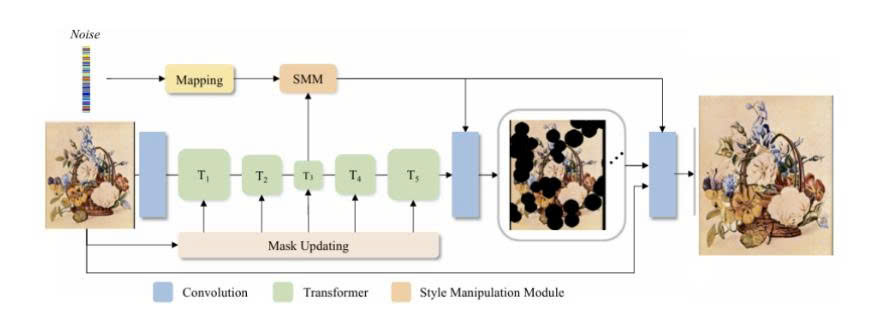
\includegraphics[width=1\linewidth]{fig3_1_pipeline.jpg}
    \caption{Overall digital artwork restoration pipeline based on the Mask-Aware Transformer.}
    \label{fig:pipeline}
\end{figure}

As illustrated in Fig.3.1, the adopted Mask-Aware Transformer (MAT) framework for artwork restoration consists of a convolutional head, a transformer-based reasoning body, a convolutional reconstruction tail, and a refinement module. This hybrid design combines the strengths of convolutional neural networks and transformer architectures, enabling both local texture modeling and long-range structural reasoning, which are critical for restoring damaged artworks.

Specifically, the convolutional head first extracts low-level visual features from the masked artwork and converts them into token representations. These tokens are then processed by the main transformer body, which is composed of multiple stages of transformer blocks operating at different spatial resolutions. Through multi-head contextual attention, the transformer body captures long-range dependencies between visible regions and missing areas, allowing the model to infer globally consistent structures such as facial contours, object boundaries, and compositional layouts commonly found in artistic images.

The output tokens from the transformer body are subsequently passed to a convolution-based reconstruction module, which progressively upsamples the feature representations to recover the original image resolution. To further enhance high-frequency details, especially painterly textures and brushstroke patterns, an additional convolutional refinement network is applied. This refinement stage leverages the efficiency and local texture modeling capability of CNNs to improve visual sharpness in the restored regions.

Overall, the adopted MAT-based framework is designed to support non-invasive digital artwork restoration. By combining global semantic reasoning with local texture refinement, the framework produces visually plausible restorations while preserving artistic structure and style, making it suitable as a decision-support tool for artwork analysis and restoration planning rather than a replacement for expert-driven physical restoration.

% ------------------------------------------------------------
\section{Convolutional Head for Artwork Restoration}

The convolutional head takes as input the degraded artwork image $I_M$ together with its corresponding binary damage mask $M$, and produces compact feature maps at $\frac{1}{8}$ of the original spatial resolution. These feature maps are then flattened into tokens and fed into the transformer body.

This module consists of four convolutional layers. The first layer adjusts the input channel dimension, while the subsequent layers progressively downsample the spatial resolution. Such a design is well-suited for artwork restoration, where early-stage preservation of local texture patterns, brushstroke orientation, and color transitions is essential.

The convolutional head is introduced for two main reasons. First, convolutional operations embed strong local inductive priors, which improve representation quality for fine-grained artistic details. Second, fast spatial downsampling significantly reduces computational complexity and memory consumption, enabling efficient processing of high-resolution artworks. Empirically, this design yields more stable optimization and higher-quality restorations than linear projection heads used in Vision Transformers.

% ------------------------------------------------------------
\section{Transformer Body}

The transformer body is responsible for modeling long-range dependencies across the artwork image. This capability is crucial for restoring large and irregular missing regions, where global structure must be inferred from distant yet semantically related contexts.

The transformer body consists of five hierarchical stages, each composed of multiple adjusted transformer blocks. A dynamically updated mask is incorporated into the attention mechanism, ensuring that information is propagated only from valid tokens.

% ------------------------------------------------------------
\subsection{Adjusted Transformer Block}

To improve training stability under large missing regions, an adjusted transformer block is employed instead of the standard transformer design. Layer normalization is removed, and residual learning is replaced by feature concatenation followed by a fully connected projection.

As illustrated in Figure~\ref{fig:transformer_stage}, the output of the multi-head contextual attention (MCA) module is concatenated with the input feature and transformed as follows:
\begin{equation}
\mathbf{X}'_{k,\ell} = \mathrm{FC}\big([\mathrm{MCA}(\mathbf{X}_{k,\ell-1}),\; \mathbf{X}_{k,\ell-1}]\big),
\end{equation}
\begin{equation}
\mathbf{X}_{k,\ell} = \mathrm{MLP}(\mathbf{X}'_{k,\ell}),
\end{equation}
where $\mathbf{X}_{k,\ell}$ denotes the output of the $\ell$-th block in the $k$-th stage.

After several transformer blocks, a convolutional layer with a global residual connection is applied to refine the feature representation. Positional embeddings are omitted, as convolutional layers sufficiently encode spatial information. This design encourages long-range interactions driven by feature similarity, which is beneficial for restoring complex artistic structures.

\begin{figure}[H]
    \centering
    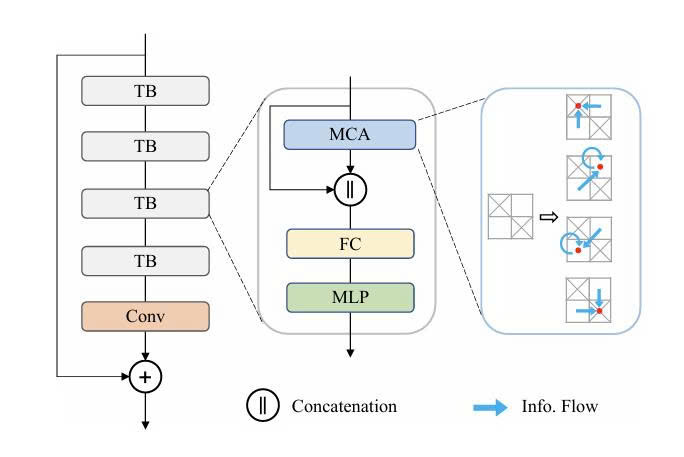
\includegraphics[width=0.9\linewidth]{mat_transformer_stage.jpg}
    \caption{Structure of a single transformer stage. ``TB'' denotes the adjusted transformer block and ``MCA'' represents multi-head contextual attention. Valid and invalid tokens are indicated by $\square$ and $\boxtimes$, respectively.}
    \label{fig:transformer_stage}
\end{figure}
Standard transformer architectures often suffer from unstable optimization when applied to images dominated by missing regions. Invalid tokens may dominate normalization statistics and residual learning tends to emphasize high-frequency details prematurely. Replacing residual learning with feature concatenation alleviates these issues and results in more stable and visually coherent restorations.

% ------------------------------------------------------------
\subsection{Multi-Head Contextual Attention}

To handle a large number of tokens with low initial fidelity, the multi-head contextual attention mechanism selectively aggregates information from valid tokens only. The attention operation is defined as:
\begin{equation}
\mathrm{Att}(\mathbf{Q}, \mathbf{K}, \mathbf{V}) =
\mathrm{Softmax}\left(\frac{\mathbf{Q}\mathbf{K}^T + \mathbf{M}'}{\sqrt{d_k}}\right)\mathbf{V},
\end{equation}
where $\mathbf{Q}$, $\mathbf{K}$, and $\mathbf{V}$ are the query, key, and value matrices, respectively.

The dynamic mask $\mathbf{M}'$ is defined as:
\begin{equation}
\mathbf{M}'_{ij} =
\begin{cases}
0, & \text{if token}_j \text{ is valid}, \\
-\tau, & \text{if token}_j \text{ is invalid},
\end{cases}
\end{equation}
where $\tau$ is a large positive constant that suppresses contributions from invalid tokens.

Window-based attention with periodic shifting is employed to balance efficiency and global information flow.

\noindent\textbf{Mask Updating Strategy.}

The validity mask is initialized from the input damage mask and updated dynamically. A window becomes valid if at least one valid token exists within it. Through repeated attention and window shifting, contextual information gradually propagates, enabling reconstruction of large damaged regions.

\begin{figure}[H]
    \centering
    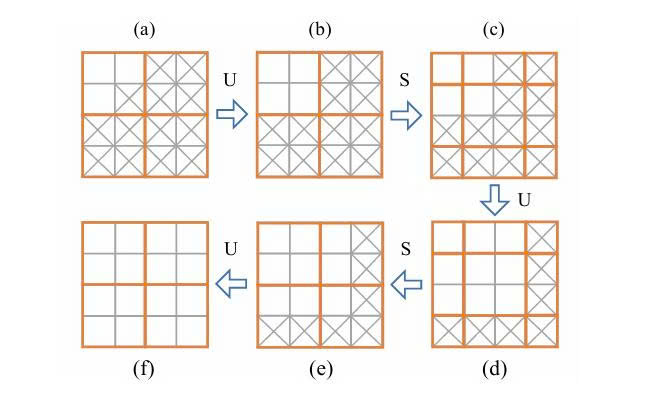
\includegraphics[width=0.7\linewidth]{mat_mask_update.jpg}
    \caption{Illustration of the dynamic mask updating strategy. Valid regions progressively expand through attention and window shifting.}
    \label{fig:mask_update}
\end{figure}

% ------------------------------------------------------------
\section{Style Manipulation Module}

Artwork restoration is inherently ambiguous, as multiple plausible reconstructions may exist for the same damaged region. To support pluralistic generation, a style manipulation module is incorporated.

A noise-unconditional style representation is first obtained:
\begin{equation}
\mathbf{s}_u = \mathcal{E}(\mathbf{n}),
\end{equation}
and combined with image features as:
\begin{equation}
\mathbf{X}' = \mathbf{B} \odot \mathbf{X} + (1-\mathbf{B}) \odot \mathrm{Resize}(\mathbf{s}_u),
\end{equation}
where $\mathbf{B}$ is a random binary mask.

The image-conditioned style is computed as:
\begin{equation}
\mathbf{s}_c = \mathcal{F}(\mathbf{X}'),
\end{equation}
and fused as:
\begin{equation}
\mathbf{s} = \mathcal{A}(\mathbf{s}_u, \mathbf{s}_c).
\end{equation}

The final style representation modulates convolution weights:
\begin{equation}
\mathbf{W}'_{ijk} = \mathbf{W}_{ijk} \cdot \mathbf{s}_i,
\end{equation}
\begin{equation}
\mathbf{W}''_{ijk} =
\frac{\mathbf{W}'_{ijk}}{\sqrt{\sum_{i,k}(\mathbf{W}'_{ijk})^2 + \epsilon}}.
\end{equation}

This mechanism enables diverse yet stylistically coherent restoration outcomes.

% ------------------------------------------------------------
\section{Loss Functions}

To ensure high perceptual quality and artistic realism, the model is optimized using a combination of adversarial and perceptual losses.

\textbf{Adversarial Loss.}
\begin{equation}
\mathcal{L}_G = -\mathbb{E}_{\hat{x}}[\log D(\hat{x})],
\end{equation}
\begin{equation}
\mathcal{L}_D = -\mathbb{E}_{x}[\log D(x)] -
\mathbb{E}_{\hat{x}}[\log (1 - D(\hat{x}))].
\end{equation}

\textbf{Perceptual Loss.}
\begin{equation}
\mathcal{L}_P =
\sum_i \eta_i \|\phi_i(\hat{x}) - \phi_i(x)\|_1,
\end{equation}
where $\phi_i(\cdot)$ denotes VGG-19 feature activations.

% ============================================================
% 3.6 Experiments and Results
% ============================================================

\section{Experiments and Results}
\label{sec:experiments_results}

This section presents the experimental setup and evaluation results of applying the
Mask-Aware Transformer (MAT) to the task of digital artwork restoration. The experiments
are designed to assess the model's ability to reconstruct large and irregularly damaged
regions in oil paintings while preserving structural integrity, painterly texture, and
stylistic coherence.

% ------------------------------------------------------------
% 3.6.1 Dataset Construction and Damage Mask Generation
% ------------------------------------------------------------

\subsection{Dataset Construction and Damage Mask Generation}
\label{sec:dataset_mask_generation}

\noindent\textbf{Artwork Dataset Collection}

To evaluate the applicability of MAT for artwork restoration, a dedicated dataset of
digitized oil paintings is constructed. The dataset primarily consists of paintings by
Vincent van Gogh, selected due to their distinctive brushstroke patterns, strong color
contrasts, and frequent use in digital art and restoration research.

Only artworks with sufficient resolution and minimal compression artifacts are retained.
Images containing watermarks, severe cropping, or excessive noise are excluded to ensure
data quality and reliability of the restoration results. All selected images are resized
to a fixed resolution of $512 \times 512$ pixels and represented in the RGB color space.

The dataset is used exclusively for evaluation purposes rather than large-scale training.

\begin{table}[H]
\centering
\caption{Summary of the Artwork Dataset}
\label{tab:dataset}
\begin{tabular}{ll}
\toprule
\textbf{Property} & \textbf{Description} \\
\midrule
Artwork type & Oil paintings \\
Artist & Vincent van Gogh \\
Image format & PNG \\
Resolution & $512 \times 512$ \\
Color space & RGB \\
Usage & Evaluation \\
\bottomrule
\end{tabular}
\end{table}

\noindent\textbf{Damage Mask Generation}

To simulate realistic artwork degradation, damage masks are applied to the original oil
paintings to generate corrupted input images. The masked regions represent missing or
degraded content caused by aging, abrasion, or physical damage commonly observed in
historical artworks.

Compared to natural-image inpainting, artwork restoration requires stricter constraints
on stylistic coherence, brushstroke continuity, and compositional integrity, particularly
under large and irregular damage patterns. Therefore, free-form irregular masks are
adopted to emulate realistic paint loss, cracks, and occlusions. These masks produce
large missing regions that challenge the model's ability to recover both global structure
and fine-grained artistic details.

The mask coverage ratio follows the large-hole inpainting setting commonly adopted in
the original MAT framework. Representative examples of simulated artwork damage are
illustrated in Figure~\ref{fig:mask_examples}.

\begin{figure}[H]
\centering
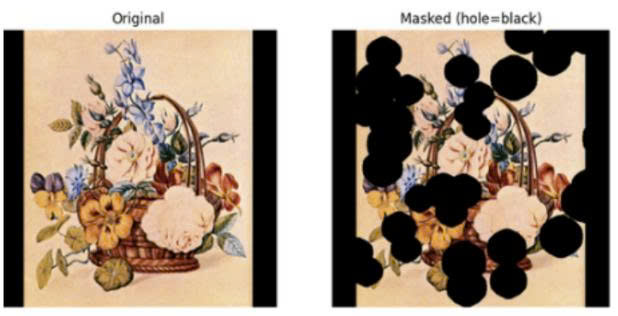
\includegraphics[width=0.85\linewidth]{fig3_2_mask_examples.jpg}
\caption{Artwork damage simulation examples using large irregular masks.}
\label{fig:mask_examples}
\end{figure}

\begin{table}[H]
\centering
\caption{Mask Statistics}
\label{tab:mask_statistics}
\begin{tabular}{ll}
\toprule
\textbf{Metric} & \textbf{Value} \\
\midrule
Mask type & Large irregular \\
Average masked area & $\sim 35\%$ \\
Minimum masked area & $\sim 20\%$ \\
Maximum masked area & $\sim 50\%$ \\
\bottomrule
\end{tabular}
\end{table}

% ------------------------------------------------------------
% 3.6.2 Experimental Results
% ------------------------------------------------------------

\subsection{Experimental Results}
\label{sec:experimental_results}

\noindent\textbf{Visual Restoration Results}

This subsection analyzes the qualitative restoration behavior of MAT when applied to
damaged oil paintings under controlled experimental settings. Visual evaluation is
conducted by comparing the original image, the masked input, and the restored output
generated by the model.

Figure~\ref{fig:visual_grid_results} presents representative restoration examples. The results
demonstrate that MAT is capable of maintaining long-range structural coherence, even
under large missing regions. The reconstructed areas exhibit painterly texture patterns
that are visually consistent with the surrounding context, suggesting effective modeling
of artistic style and brushstroke continuity.

Despite these strengths, minor artifacts may still appear near complex brushstroke
boundaries or in regions with highly ambiguous texture patterns. These limitations
highlight the inherent difficulty of artwork restoration and motivate further refinement
in handling fine-grained artistic details.

\begin{figure}[H]
\centering

% ----- Header row (optional): dùng text thay vì ảnh -----
\begin{minipage}{0.32\linewidth}\centering \textbf{Original}\end{minipage}
\begin{minipage}{0.32\linewidth}\centering \textbf{Masked (hole = black)}\end{minipage}
\begin{minipage}{0.32\linewidth}\centering \textbf{Output}\end{minipage}
\vspace{0.3em}

% ----- Row 1 -----
\begin{minipage}{0.32\linewidth}\centering
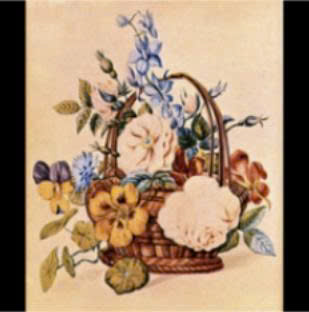
\includegraphics[width=\linewidth]{ex1_original.jpg}
\end{minipage}
\begin{minipage}{0.32\linewidth}\centering
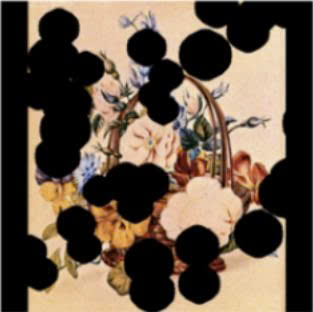
\includegraphics[width=\linewidth]{ex1_masked.jpg}
\end{minipage}
\begin{minipage}{0.32\linewidth}\centering

\includegraphics[width=\linewidth]{ex1_output.jpg}
\end{minipage}
\vspace{0.4em}

% ----- Row 2 -----
\begin{minipage}{0.32\linewidth}\centering
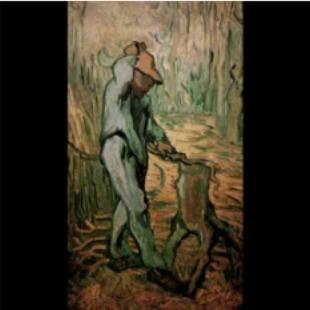
\includegraphics[width=\linewidth]{ex2_original.jpg}
\end{minipage}
\begin{minipage}{0.32\linewidth}\centering
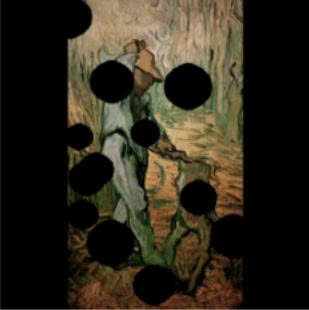
\includegraphics[width=\linewidth]{ex2_masked.jpg}
\end{minipage}
\begin{minipage}{0.32\linewidth}\centering
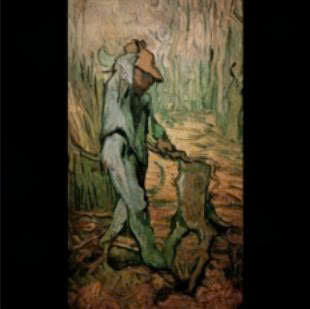
\includegraphics[width=\linewidth]{ex2_output.jpg}
\end{minipage}
\vspace{0.4em}

% ----- Row 3 -----
\begin{minipage}{0.32\linewidth}\centering
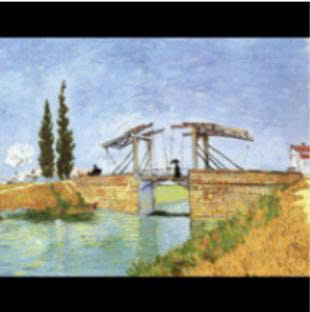
\includegraphics[width=\linewidth]{ex3_original.jpg}
\end{minipage}
\begin{minipage}{0.32\linewidth}\centering
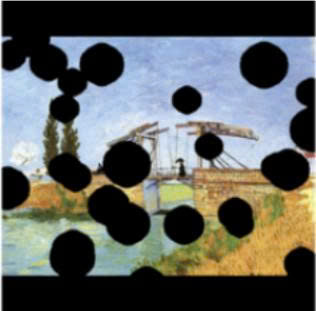
\includegraphics[width=\linewidth]{ex3_masked.jpg}
\end{minipage}
\begin{minipage}{0.32\linewidth}\centering
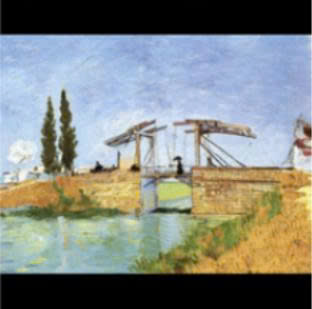
\includegraphics[width=\linewidth]{ex3_output.jpg}
\end{minipage}
\vspace{0.4em}

% ----- Row 4 -----
\begin{minipage}{0.32\linewidth}\centering
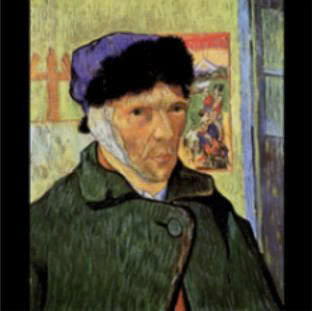
\includegraphics[width=\linewidth]{ex4_original.jpg}
\end{minipage}
\begin{minipage}{0.32\linewidth}\centering
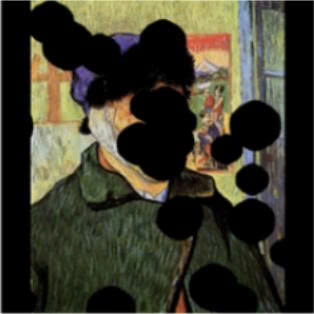
\includegraphics[width=\linewidth]{ex4_masked.jpg}
\end{minipage}
\begin{minipage}{0.32\linewidth}\centering
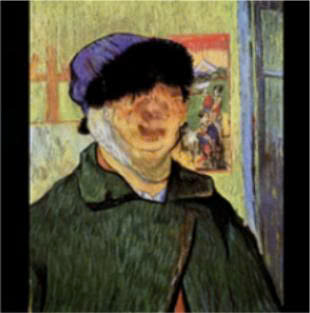
\includegraphics[width=\linewidth]{ex4_output.jpg}
\end{minipage}

\caption{Visual comparison of restoration results (original, masked input, and MAT-restored output).}
\label{fig:visual_grid_results}
\end{figure}



\section{Proposed Improvements}

This section outlines potential directions for the official thesis and does not propose a new inpainting model. All improvements are designed to extend or adapt the existing MAT framework for artwork restoration.

\subsection{Face-Oriented Artwork Restoration and Sharpness Enhancement}

\begin{figure}[H]
    \centering
    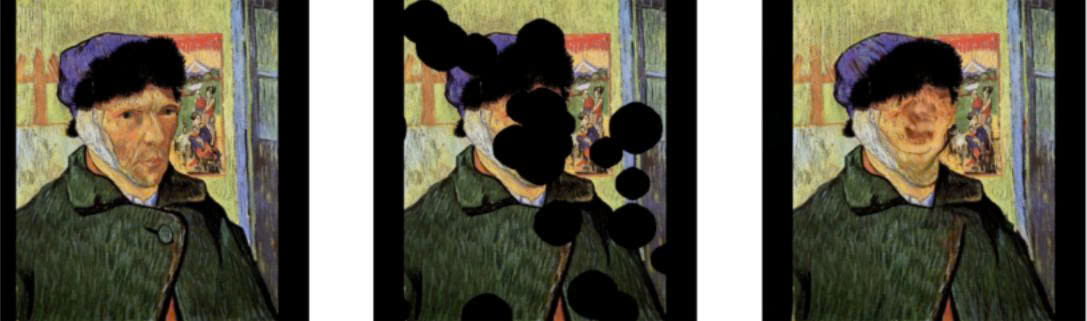
\includegraphics[width=1\linewidth]{fig3_7_face_limitation.jpg}
    \caption{Limitation of MAT in face restoration for oil paintings.}
    \label{fig:face_limitation}
\end{figure}

A particularly important direction for extending the methodology is the restoration of human faces in oil paintings, where perceptual sensitivity and visual accuracy are significantly higher than in background regions.

Although global facial structure is reasonably reconstructed, fine-grained texture details are often over-smoothed, resulting in blurred facial features. Human observers are especially sensitive to such artifacts.

Future extensions will focus on portrait-dominated datasets, region-aware evaluation, and perceptual loss functions correlated with facial structure preservation.

\subsection{Realistic Damage Modeling}

More realistic damage masks can be introduced to better reflect real-world artwork degradation, including:
\begin{itemize}
    \item Craquelure patterns caused by aging paint layers
    \item Thin crack networks
    \item Progressive paint loss with irregular boundaries
\end{itemize}

\subsection{High-Resolution Artwork Restoration}

Future research may explore patch-based or multi-scale inference strategies to support ultra-high-resolution artworks while maintaining global consistency.

\subsection{Integration of Structural Priors}

Incorporating lightweight structural priors, such as edge or contour guidance, may further improve line continuity and structural accuracy in regions with strong geometric patterns.

\section{Summary}

This chapter presented the methodological framework for applying the Mask-Aware Transformer (MAT) to digital artwork restoration. An inference-driven pipeline was designed, covering artwork dataset preparation, realistic damage mask generation, MAT-based inpainting, and perceptually aligned evaluation criteria. The methodology emphasizes non-invasive restoration and adapts MAT to the artistic domain without introducing new model architectures.

\fi

% =========================
% Bibliography (placeholder)
% =========================
\nocite{*}
\bibliographystyle{ieeetr}
\bibliography{reference}


\end{document}


